\documentclass[a4paper,12pt]{article}
\usepackage{geometry}
\geometry{left=3cm,right=3cm,top=3cm,bottom=3cm,footskip=2cm}
\usepackage{setspace}	
\linespread{1.3}

\usepackage{lmodern}
\usepackage{amssymb,amsmath}
%\usepackage{ifxetex,ifluatex}
%\usepackage{fixltx2e} % provides \textsubscript
\usepackage[T1]{fontenc}
\usepackage[utf8]{inputenc}
\usepackage{eurosym}
%\usepackage{natbib}
%\bibliographystyle{plainnat}
%\usepackage{biblatex}
%\bibliography{}
\usepackage{listings}
%Allow degree escape in listings
\usepackage{gensymb}
\lstnewenvironment{code}{\lstset{language=Haskell,basicstyle=\small\ttfamily}}{}
\usepackage{color}
\usepackage{fancyvrb}
\newcommand{\VerbBar}{|}
\newcommand{\VERB}{\Verb[commandchars=\\\{\}]}
\DefineVerbatimEnvironment{Highlighting}{Verbatim}{commandchars=\\\{\}}
% Add ',fontsize=\small' for more characters per line
\newenvironment{Shaded}{}{}
\newcommand{\KeywordTok}[1]{\textcolor[rgb]{0.00,0.44,0.13}{\textbf{{#1}}}}
\newcommand{\DataTypeTok}[1]{\textcolor[rgb]{0.56,0.13,0.00}{{#1}}}
\newcommand{\DecValTok}[1]{\textcolor[rgb]{0.25,0.63,0.44}{{#1}}}
\newcommand{\BaseNTok}[1]{\textcolor[rgb]{0.25,0.63,0.44}{{#1}}}
\newcommand{\FloatTok}[1]{\textcolor[rgb]{0.25,0.63,0.44}{{#1}}}
\newcommand{\ConstantTok}[1]{\textcolor[rgb]{0.53,0.00,0.00}{{#1}}}
\newcommand{\CharTok}[1]{\textcolor[rgb]{0.25,0.44,0.63}{{#1}}}
\newcommand{\SpecialCharTok}[1]{\textcolor[rgb]{0.25,0.44,0.63}{{#1}}}
\newcommand{\StringTok}[1]{\textcolor[rgb]{0.25,0.44,0.63}{{#1}}}
\newcommand{\VerbatimStringTok}[1]{\textcolor[rgb]{0.25,0.44,0.63}{{#1}}}
\newcommand{\SpecialStringTok}[1]{\textcolor[rgb]{0.73,0.40,0.53}{{#1}}}
\newcommand{\ImportTok}[1]{{#1}}
\newcommand{\CommentTok}[1]{\textcolor[rgb]{0.38,0.63,0.69}{\textit{{#1}}}}
\newcommand{\DocumentationTok}[1]{\textcolor[rgb]{0.73,0.13,0.13}{\textit{{#1}}}}
\newcommand{\AnnotationTok}[1]{\textcolor[rgb]{0.38,0.63,0.69}{\textbf{\textit{{#1}}}}}
\newcommand{\CommentVarTok}[1]{\textcolor[rgb]{0.38,0.63,0.69}{\textbf{\textit{{#1}}}}}
\newcommand{\OtherTok}[1]{\textcolor[rgb]{0.00,0.44,0.13}{{#1}}}
\newcommand{\FunctionTok}[1]{\textcolor[rgb]{0.02,0.16,0.49}{{#1}}}
\newcommand{\VariableTok}[1]{\textcolor[rgb]{0.10,0.09,0.49}{{#1}}}
\newcommand{\ControlFlowTok}[1]{\textcolor[rgb]{0.00,0.44,0.13}{\textbf{{#1}}}}
\newcommand{\OperatorTok}[1]{\textcolor[rgb]{0.40,0.40,0.40}{{#1}}}
\newcommand{\BuiltInTok}[1]{{#1}}
\newcommand{\ExtensionTok}[1]{{#1}}
\newcommand{\PreprocessorTok}[1]{\textcolor[rgb]{0.74,0.48,0.00}{{#1}}}
\newcommand{\AttributeTok}[1]{\textcolor[rgb]{0.49,0.56,0.16}{{#1}}}
\newcommand{\RegionMarkerTok}[1]{{#1}}
\newcommand{\InformationTok}[1]{\textcolor[rgb]{0.38,0.63,0.69}{\textbf{\textit{{#1}}}}}
\newcommand{\WarningTok}[1]{\textcolor[rgb]{0.38,0.63,0.69}{\textbf{\textit{{#1}}}}}
\newcommand{\AlertTok}[1]{\textcolor[rgb]{1.00,0.00,0.00}{\textbf{{#1}}}}
\newcommand{\ErrorTok}[1]{\textcolor[rgb]{1.00,0.00,0.00}{\textbf{{#1}}}}
\newcommand{\NormalTok}[1]{{#1}}
\usepackage{longtable,booktabs}
\usepackage{graphicx}
\usepackage{pdfpages}
\makeatletter
\def\maxwidth{\ifdim\Gin@nat@width>\linewidth\linewidth\else\Gin@nat@width\fi}
\def\maxheight{\ifdim\Gin@nat@height>\textheight\textheight\else\Gin@nat@height\fi}
\makeatother
% Scale images if necessary, so that they will not overflow the page
% margins by default, and it is still possible to overwrite the defaults
% using explicit options in \includegraphics[width, height, ...]{}
\setkeys{Gin}{width=\maxwidth,height=\maxheight,keepaspectratio}
\usepackage[unicode=true]{hyperref}
\hypersetup{breaklinks=true,
            bookmarks=true,
            pdfauthor=Esteban Munoz,
            pdftitle=Guidelines Energy-ADE,
            colorlinks=true,
            citecolor=blue,
            urlcolor=blue,
            linkcolor=magenta,
            pdfborder={0 0 0}}
\urlstyle{same}  % don't use monospace font for urls
% Make links footnotes instead of hotlinks:
\renewcommand{\href}[2]{#2\footnote{\url{#1}}}
\setlength{\parindent}{0pt}
\setlength{\parskip}{6pt plus 2pt minus 1pt}
\setlength{\emergencystretch}{3em}  % prevent overfull lines
%%\setcounter{secnumdepth}{0}
%
\usepackage{enumitem}
\setlist{nosep, noitemsep}

\providecommand{\tightlist}{%
  \setlength{\itemsep}{0pt}\setlength{\parskip}{0pt}}

%% Reformat Sections
\let\stdsection\section%
\renewcommand\section{\newpage\stdsection}

%% Title Page
\usepackage{fancyhdr}
\pagestyle{fancy}
\fancyhf{}

%% Normal page
\fancypagestyle{normalpage}{%
\fancyhf{}
\rhead{%
    \begin{footnotesize}
        ADE Energy Core
    \end{footnotesize}
}
\lfoot{%
    \begin{footnotesize}
        {}
    \end{footnotesize}
    }
\rfoot{%
    \begin{footnotesize}
        \thepage%
    \end{footnotesize}
}
\renewcommand{\headrulewidth}{0pt} % remove lines as well
\renewcommand{\footrulewidth}{0pt}
\renewcommand{\headwidth}{17cm}
}

%% Title Page
\fancypagestyle{titlepage}{%
\fancyhf{}
% The title page has different margins 
\renewcommand{\headrulewidth}{0pt} % remove lines as well
\renewcommand{\footrulewidth}{0pt}
}

\pagestyle{titlepage}
\usepackage{color}
\definecolor{lightgray}{gray}{0.60}
%% Maketitle
\renewcommand\maketitle{%
\sffamily
\begin{flushright}

\includegraphics[width=4cm]{./fig/logo.png}
\end{flushright}
    \thispagestyle{titlepage}
    \vspace{3.4cm}
    {\noindent \textcolor{lightgray}{Draft Guidelines - Energy ADE version 0.7} \par}
    \vspace{0.3cm}
    {\noindent \large \bfseries CityGML Energy Application Domain Extension \par}
    \vspace{0.7cm}
    {\noindent In collaboration with OGC and SIG 3D \par}
    \vspace{0.7cm}
    {\noindent \textcolor{lightgray}{\today} \par}
\newpage
\begin{flushleft}
\begin{tabular}{lll}
    \toprule
    \textbf{Revision updates} & \textbf{When} & \textbf{Who}\\
    \midrule
    Basis version &
    03.08.2015 &
    RN
\\
    Markdown export &
    22.10.2015 &
    EM
%    Basis version\\Markdown export 
    \\
    \bottomrule
\end{tabular}
\end{flushleft}
\textbf{Authors:}\\
{\noindent \normalsize \normalfont%
}
\par
\vspace{0.3cm}
\textbf{Consortium participating institutes:}
\begin{itemize}
    \itemsep-1.3em
    \item University of Applied Sciences Stuttgart, Germany\\\item Technische Universität München, Germany\\\item Karlsruhe Institute für Technologie, Germany\\\item European Institute for Energy Research, Germany\\\item RWTH Aachen University / E.ON Energy Research Center, Germany\\\item HafenCity Universität Hamburg, Germany\\\item Ecole Polytechnique Fédérale de Lausanne, Switzerland\\\item Centre Scientifique et Technique du Batiment, France\\\item Electricité de France, France\\\item Sinergis, Italy\\\item M.O.S.S Computer Grafik Systeme, Germany\\\item Austrian Institute of Technology, Austria
\end{itemize}
\newpage
}

% show only two levels in the table of content
\setcounter{tocdepth}{2}

\begin{document}
\pagestyle{titlepage}
\maketitle
\pagestyle{normalpage}
\begin{abstract}
The Energy Application Domain Extension (Energy ADE) described in this
documentation defines a standardized data model based on the CityGML 2.0
format for urban energy analyses, aiming to be a reference exchange data
model between different urban modelling tools and expert databases.

The Energy ADE has been developed since May 2014 by an international
consortium of urban energy simulation developers and users, both
academic and commercial. To date, the consortium is composed by:
University of Applied Sciences Stuttgart, Technische Universität
München, Karlsruhe Institute für Technologie, RWTH Aachen University /
E.ON Energy Research Center, HafenCity Universität Hamburg, European
Institute for Energy Research, Ecole Polytechnique Fédérale de Lausanne,
Centre Scientifique et Technique du Batiment, Electricité de France,
Sinergis, M.O.S.S Computer Grafik Systeme and Austrian Institute of
Technology.
\end{abstract}
\newpage
\pagestyle{normalpage}


\hypersetup{linkcolor=black}
\tableofcontents
\newpage
\section{Overview of the Energy Application Domain
Extension}\label{overview-of-the-energy-application-domain-extension}

The CityGML Energy Application Domain Extension (Energy ADE) aims at
extending the CityGML 2.0 standard with energy-related entities and
attributes necessary to perform energy analyses at urban scale.

In accordance with the philosophy of CityGML, the Energy ADE aims to be
flexible in terms of compatibility with different data qualities, levels
of detail and urban energy model complexities (e.g.~from monthly energy
balance methods as of ISO 13790, to sub-hourly dynamic simulations by
means of software programs like CitySim or EnergyPlus). It intends also
to take into consideration the INSPIRE Directive of the European
Parliament, as well as the recent US Building Energy Data Exchange
Specification (BEDES).

Its structure is conceived to be modular. In its current version 0.7, it
consists of 5 modules:

\begin{itemize}
\tightlist
\item
  Building Physics module,
\item
  Occupancy module,
\item
  Construction and Material module,
\item
  Energy System module,
\item
  Timeseries and Schedules module.
\end{itemize}

Some modules can be potentially used and extended also for other
applications (e.g.~module Occupancy for socio-economics, module
Construction and Materials for acoustics or statics, etc).

This document is intended to explain the characteristics and purposes of
each module, their entities and attributes. It provides also a number of
XML examples, illustrating how and where the Energy ADE entities and
attributes may be embedded into CityGML.

\section{Building Physics Module}\label{building-physics-module}

\subsection{Module overview and main
relationships}\label{module-overview-and-main-relationships}

This module contains the thermal building objects required for building
thermal modelling (e.g.~calculation of space heating and space cooling
demands): \texttt{ThermalZone}, \texttt{ThermalBoundary},
\texttt{ThermalComponent}. These thermal building objects are linked to
the CityGML building objects through its \texttt{\_AbstractBuilding},
\texttt{\_BoundarySurface}, \texttt{\_Opening} classes, which are
extended with Energy ADE attributes.

The \texttt{ThermalZone}, which represents the spatial unit for heating
and cooling demand calculation, is the central object of this Building
Physics Module. A Building may have several \texttt{ThermalZone}, for
instance in the case of mixed-usage building, or to distinguish rooms or
zones with different solar gains and/or thermal behaviour.

If occupied, a \texttt{ThermalZone} must be related to at less 1
\texttt{UsageZone}, which contains the usage boundary conditions for the
heating and cooling demand calculation (see Occupancy Module).
\texttt{ThermalZone} may be related to several \texttt{UsageZone} for
simplified modelling of mixed-usage space, in which case the usage
boundary conditions of the \texttt{UsageZone} should be aggregated or
weighted according with their floorArea.

These \texttt{ThermalZone} objects are separated from each other and
from the outside by \texttt{ThermalBoundary} objects. These
\texttt{ThermalBoundary} objects may or not correspond to the CityGML
\texttt{\_BoundarySurface}. However, every \texttt{ThermalBoundary}
delimiting the \texttt{ThermalZone} from outside must be related
(\texttt{correspondsTo}) with a \texttt{\_BoundarySurface}, in order to
consider the \texttt{globalSolarIrradiance} incident on
\texttt{\_BoundarySurface} in the heating and cooling calculations.

\subsection{Building, zones and
boundaries}\label{building-zones-and-boundaries}

\begin{figure}[htbp]
\centering
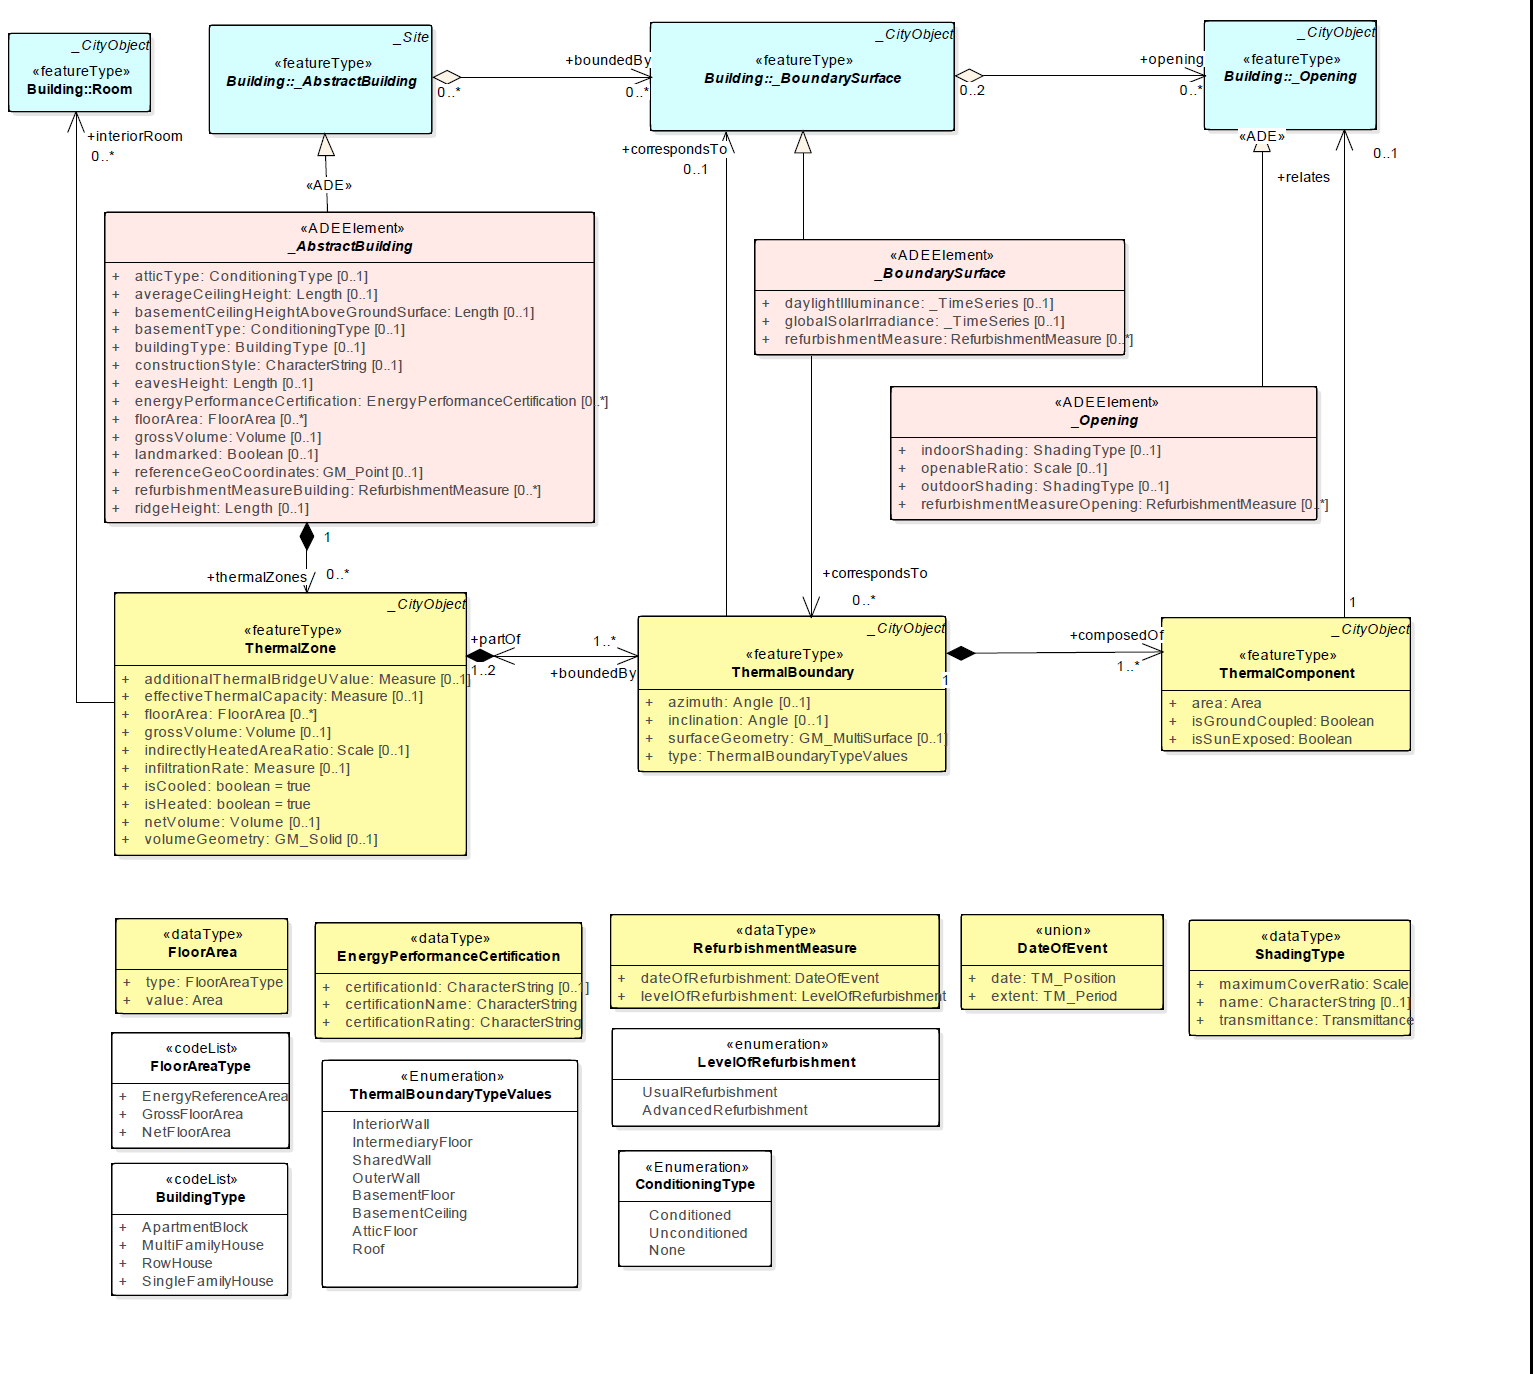
\includegraphics{fig/class_geometry.png}
\caption{Class diagram of Building Physics Module}
\end{figure}

\subsubsection{\_AbstractBuilding}\label{abstractbuilding}

The Energy ADE extends the CityGML \_AbstractBuilding by a number of
energy-related attributes, e.g with regards to the geometrical
characteristics (\texttt{referencePoint}, \texttt{averageCeilingHeight},
\texttt{eavesHeight}, \texttt{ridgeHeight},
\texttt{basementCeilingHeightAboveGrounSurface}, \texttt{floorArea},
\texttt{grossVolume}), to the conditioning of basement and attic
(\texttt{basementType}, \texttt{atticType}), to the available energy
certificates (\texttt{energyPerformanceCertification}) and refurbishment
measures (\texttt{RefurbishmentMeasureOnBuilding}), and other building
information useful for building typology categorisations
(\texttt{buildingType} and \texttt{constructionStyle}).

All these attributes are optional. Some of them, like \texttt{floorArea}
and\\
\texttt{energyPerformanceCertification}, have a cardinality {[}0..*{]}
and may consequently be attributed several times to a building,
specifying different values for different \texttt{FloorAreaType},
respectively \texttt{certificationName}.

Finally, because \texttt{\_AbstractBuilding} inherits from
\texttt{\_CityObject}, further objects may be assigned to it, like
\texttt{EnergyDemand} in particular (see Module Energy and Systems).

In the following, an extract of CityGML file for a building is given,
included some of its Energy ADE attributes.

\begin{Shaded}
\begin{Highlighting}[]
\CommentTok{<!--Examples of Building with Energy ADE attributes-->}
\KeywordTok{<bldg:Building}\OtherTok{ gml:id=}\StringTok{"id_building_1"}\KeywordTok{>}
    \KeywordTok{<gml:description>}\NormalTok{Description of Building 1}\KeywordTok{</gml:description>}
    \KeywordTok{<gml:name>}\NormalTok{Name of Building 1}\KeywordTok{</gml:name>}
    \KeywordTok{<energy:referencePoint>}
        \KeywordTok{<gml:Point}\OtherTok{ gml:id=}\StringTok{"id_building_referencepoint_1"}\OtherTok{ srsName=}\StringTok{"EPSG:31256"}\OtherTok{ srsDimension=}\StringTok{"3"}\KeywordTok{>}
            \KeywordTok{<gml:pos>}\NormalTok{5 5 0}\KeywordTok{</gml:pos>}
        \KeywordTok{</gml:Point>}
    \KeywordTok{</energy:referencePoint>}
    \KeywordTok{<energy:basementType>}\NormalTok{Unconditioned}\KeywordTok{</energy:basementType>}
    \KeywordTok{<energy:energyPerformanceCertification>}
        \CommentTok{<!--Here come the EnergyPerformanceCertification objects (see later) -->}
    \KeywordTok{</energy:energyPerformanceCertification>}
    \KeywordTok{<energy:basementCeilingHeightAboveGroundSurface}\OtherTok{ uom=}\StringTok{"m"}\KeywordTok{>}\NormalTok{1}\KeywordTok{</energy:basementCeilingHeightAboveGroundSurface>}
    \KeywordTok{<energy:grossVolume}\OtherTok{ uom=}\StringTok{"m^3"}\KeywordTok{>}\NormalTok{1050}\KeywordTok{</energy:grossVolume>}
    \KeywordTok{<energy:refurbishmentMeasureOnBuilding>}
        \KeywordTok{<energy:RefurbishmentMeasure>}
            \CommentTok{<!--Here come all attributes of a RefurbishmentMeasure object (omitted here)-->}
        \KeywordTok{</energy:RefurbishmentMeasure>}
    \KeywordTok{</energy:refurbishmentMeasureOnBuilding>}
    \KeywordTok{<energy:averageCeilingHeight}\OtherTok{ uom=}\StringTok{"m"}\KeywordTok{>}\NormalTok{2.7}\KeywordTok{</energy:averageCeilingHeight>}
    \KeywordTok{<energy:atticType>}\NormalTok{Conditioned}\KeywordTok{</energy:atticType>}

    \CommentTok{<!--Here may come a list of UsageZone of the building (see Module Occupancy) -->}

    \KeywordTok{<energy:ridgeHeight}\OtherTok{ uom=}\StringTok{"m"}\KeywordTok{>}\NormalTok{10.5}\KeywordTok{</energy:ridgeHeight>}
    \KeywordTok{<energy:landmarked>}\NormalTok{false}\KeywordTok{</energy:landmarked>}
    \KeywordTok{<energy:floorArea>}
        \CommentTok{<!--Here come the floorArea objects (see later)-->}
    \KeywordTok{</energy:floorArea>}
    \KeywordTok{<energy:eavesHeight}\OtherTok{ uom=}\StringTok{"m"}\KeywordTok{>}\NormalTok{8}\KeywordTok{</energy:eavesHeight>}
    \KeywordTok{<energy:constructionStyle>}\NormalTok{Massive}\KeywordTok{</energy:constructionStyle>}
    \KeywordTok{<energy:buildingType>}\NormalTok{MultiFamilyHouse}\KeywordTok{</energy:buildingType>}

    \CommentTok{<!--Here follow all ThermalZone objects, each inside a "thermalZones" tag-->}
    \KeywordTok{<energy:thermalZones>}
        \KeywordTok{<energy:ThermalZone}\OtherTok{ gml:id=}\StringTok{"id_thermalzone_1"}\KeywordTok{>}
            \CommentTok{<!--Here come all attributes of the first ThermalZone (omitted here)-->}
        \KeywordTok{</energy:ThermalZone>}
    \KeywordTok{</energy:thermalZones>}
    \KeywordTok{<energy:thermalZones>}
        \KeywordTok{<energy:ThermalZone}\OtherTok{ gml:id=}\StringTok{"id_thermalzone_2"}\KeywordTok{>}
            \CommentTok{<!--Here come all attributes of the second ThermalZone (omitted here)-->}
        \KeywordTok{</energy:ThermalZone>}
    \KeywordTok{</energy:thermalZones>}
\KeywordTok{</bldg:Building>}
\end{Highlighting}
\end{Shaded}

\paragraph{FloorArea}\label{floorarea}

Buildings (\texttt{\_AbstractBuilding}) and building zones
(\texttt{ThermalZone} and \texttt{UsageZone}) may have several
\texttt{floorArea}, related to several \texttt{FloorAreaType} (e.g.~net
floor area, gross floor area, energy reference area).

\begin{Shaded}
\begin{Highlighting}[]
\CommentTok{<!--Examples of three floor areas-->}
\KeywordTok{<energy:FloorArea>}
    \KeywordTok{<energy:FloorArea>}
        \KeywordTok{<energy:type>}\NormalTok{GrossFloorArea}\KeywordTok{</energy:type>}
        \KeywordTok{<energy:value}\OtherTok{ uom=}\StringTok{"m^2"}\KeywordTok{>}\NormalTok{50.0}\KeywordTok{</energy:value>}
    \KeywordTok{</energy:FloorArea>}
    \KeywordTok{<energy:FloorArea>}
        \KeywordTok{<energy:type>}\NormalTok{NetFloorArea}\KeywordTok{</energy:type>}
        \KeywordTok{<energy:value}\OtherTok{ uom=}\StringTok{"m^2"}\KeywordTok{>}\NormalTok{40.0}\KeywordTok{</energy:value>}
    \KeywordTok{</energy:FloorArea>}
    \KeywordTok{<energy:FloorArea>}
        \KeywordTok{<energy:type>}\NormalTok{EnergyReferenceArea}\KeywordTok{</energy:type>}
        \KeywordTok{<energy:value}\OtherTok{ uom=}\StringTok{"m^2"}\KeywordTok{>}\NormalTok{43.0}\KeywordTok{</energy:value>}
    \KeywordTok{</energy:FloorArea>}
\KeywordTok{</energy:FloorArea>}
\end{Highlighting}
\end{Shaded}

\paragraph{EnergyPerformanceCertification}\label{energyperformancecertification}

A building may present several\\
\texttt{energyPerformanceCertification} related to different
\texttt{certificationName} (e.g.~PassivHaus, LEED) and/or different
certification dates (specificied by \texttt{certificationId}).

\begin{Shaded}
\begin{Highlighting}[]
\CommentTok{<!--Example of two energy performance certifications-->}
\KeywordTok{<energy:energyPerformanceCertification>}
    \KeywordTok{<energy:EnergyPerformanceCertification>}
        \KeywordTok{<energy:certificationRating>}\NormalTok{Platinum}\KeywordTok{</energy:certificationRating>}
        \KeywordTok{<energy:certificationName>}\NormalTok{LEED}\KeywordTok{</energy:certificationName>}
        \KeywordTok{<energy:certificationId>}\NormalTok{0815}\KeywordTok{</energy:certificationId>}
    \KeywordTok{</energy:EnergyPerformanceCertification>}
    \KeywordTok{<energy:EnergyPerformanceCertification>}
        \KeywordTok{<energy:certificationRating>}\NormalTok{Passive house}\KeywordTok{</energy:certificationRating>}
        \KeywordTok{<energy:certificationName>}\NormalTok{EnerPHit}\KeywordTok{</energy:certificationName>}
        \KeywordTok{<energy:certificationId>}\NormalTok{4756}\KeywordTok{</energy:certificationId>}
    \KeywordTok{</energy:EnergyPerformanceCertification>}
\KeywordTok{</energy:energyPerformanceCertification>}
\end{Highlighting}
\end{Shaded}

\paragraph{RefurbishmentMeasure}\label{refurbishmentmeasure}

Energy-efficient refurbishment operations and measures may be indicated
as attribute of \texttt{\_AbstractBuilding}, \texttt{\_BoundarySurface}
and \texttt{\_Opening}. The \texttt{RefurbishmentMeasure} object
contains two information: the date and level of refurbishment.

The attribute \texttt{levelOfRefurbishment} is a codeList whose elements
generally relates to refurbishment measure libraries or to a building
typology categorisation.

The attribute \texttt{dateOfRefurbishment} is defined by the GML type
\texttt{DateOfEvent}, and may consequently be specified in different
manners (see the 3 examples below).

\begin{Shaded}
\begin{Highlighting}[]
\CommentTok{<!--Example of a Refurbishment Measure on a building with a very vague date ("before June 2010") -->}
\KeywordTok{<energy:refurbishmentMeasureOnBuilding>}
    \KeywordTok{<energy:RefurbishmentMeasure>}
        \KeywordTok{<energy:dateOfRefurbishment>}
            \KeywordTok{<energy:DateOfEvent>}
                \KeywordTok{<energy:instant}\OtherTok{ indeterminatePosition=}\StringTok{"before"}\KeywordTok{>}\NormalTok{2010-06}\KeywordTok{</energy:instant>}
            \KeywordTok{</energy:DateOfEvent>}
        \KeywordTok{</energy:dateOfRefurbishment>}
        \KeywordTok{<energy:levelOfRefurbishment>}\NormalTok{UsualRefurbishment}\KeywordTok{</energy:levelOfRefurbishment>}
        \KeywordTok{<gml:description>}\NormalTok{Refurbishment consisting in the outside insulation of walls with 12cm polystyrol etc.}\KeywordTok{</gml:description>}
    \KeywordTok{</energy:RefurbishmentMeasure>}
\KeywordTok{</energy:refurbishmentMeasureOnBuilding>}
\end{Highlighting}
\end{Shaded}

\begin{Shaded}
\begin{Highlighting}[]
\CommentTok{<!--Example of an advanced Refurbishment Measure in the years 1998 and 1999 -->}
\KeywordTok{<energy:refurbishmentMeasureOnBuilding>}
    \KeywordTok{<energy:RefurbishmentMeasure>}
        \KeywordTok{<energy:dateOfRefurbishment>}
            \KeywordTok{<energy:DateOfEvent>}
                \KeywordTok{<energy:period>}
                    \KeywordTok{<gml:TimePeriod>}
                        \KeywordTok{<gml:beginPosition>}\NormalTok{1998}\KeywordTok{</gml:beginPosition>}
                        \KeywordTok{<gml:endPosition>}\NormalTok{2000}\KeywordTok{</gml:endPosition>}
                    \KeywordTok{</gml:TimePeriod>}
                \KeywordTok{</energy:period>}
            \KeywordTok{</energy:DateOfEvent>}
        \KeywordTok{</energy:dateOfRefurbishment>}
        \KeywordTok{<energy:levelOfRefurbishment>}\NormalTok{AdvancedRefurbishment}\KeywordTok{</energy:levelOfRefurbishment>}
    \KeywordTok{</energy:RefurbishmentMeasure>}
\KeywordTok{</energy:refurbishmentMeasureOnBuilding>}
\end{Highlighting}
\end{Shaded}

\begin{Shaded}
\begin{Highlighting}[]
\CommentTok{<!--Example of an usual Refurbishment Measure in June 2012 -->}
\KeywordTok{<energy:refurbishmentMeasureOnBuilding>}
    \KeywordTok{<energy:RefurbishmentMeasure>}
        \KeywordTok{<energy:dateOfRefurbishment>}
            \KeywordTok{<energy:DateOfEvent>}
                \KeywordTok{<energy:instant>}\NormalTok{2012-06}\KeywordTok{</energy:instant>}
            \KeywordTok{</energy:DateOfEvent>}
        \KeywordTok{</energy:dateOfRefurbishment>}
        \KeywordTok{<energy:levelOfRefurbishment>}\NormalTok{UsualRefurbishment}\KeywordTok{</energy:levelOfRefurbishment>}
    \KeywordTok{</energy:RefurbishmentMeasure>}
\KeywordTok{</energy:refurbishmentMeasureOnBuilding>}
\end{Highlighting}
\end{Shaded}

\subsubsection{\_Opening}\label{opening}

The CityGML abstract class \texttt{\_Opening} (inherited by the objects
\texttt{Window} and \texttt{Door}) is extended in this Energy ADE by a
number of energy-related attributes.

First of all, an optional attribute \texttt{openableRatio} details the
proportion of the opening area which may be opened. An indoor and an
outdoor shading system may complement the opening, with a
\texttt{ShadingType} characterized by a \texttt{transmittance} (see
details in Module Materials and Constructions) and a
\texttt{maximumCoverRatio}. Finally, information about possible
refurbishment measures and operations may also be added at the level of
the opening (e.g window exchange), through the attribute
\texttt{refurbishmentMeasureOnOpening} of type
\texttt{RefurbishmentMeasure}.

As in the Building example shown before, the standard CityGML attributes
have been omitted for better readability. The door example is simpler
and contains also information about construction and construction
orientation (by means of Xlinks).

\begin{Shaded}
\begin{Highlighting}[]
\CommentTok{<!--Example of a Window object -->}
\KeywordTok{<bldg:Window}\OtherTok{ gml:id=}\StringTok{"id_window_1"}\KeywordTok{>}
    \KeywordTok{<gml:description>}\NormalTok{This is window with an outside rolling shutter and curtains inside}\KeywordTok{</gml:description>}
    \KeywordTok{<gml:name>}\NormalTok{Window with rolling shutter and curtains}\KeywordTok{</gml:name>}

    \KeywordTok{<energy:outdoorShading>}
        \KeywordTok{<energy:ShadingType>}
            \KeywordTok{<energy:maximumCoverRatio}\OtherTok{ uom=}\StringTok{"ratio"}\KeywordTok{>}\NormalTok{1}\KeywordTok{</energy:maximumCoverRatio>}
            \KeywordTok{<energy:name>}\NormalTok{Rolling shutter}\KeywordTok{</energy:name>}
            \KeywordTok{<energy:transmittance>}
                \KeywordTok{<energy:Transmittance>}
                    \KeywordTok{<energy:fraction}\OtherTok{ uom=}\StringTok{"ratio"}\KeywordTok{>}\NormalTok{0}\KeywordTok{</energy:fraction>}
                    \KeywordTok{<energy:wavelengthRange>}\NormalTok{Total}\KeywordTok{</energy:wavelengthRange>}
                \KeywordTok{</energy:Transmittance>}
            \KeywordTok{</energy:transmittance>}
        \KeywordTok{</energy:ShadingType>}
    \KeywordTok{</energy:outdoorShading>}

    \KeywordTok{<energy:indoorShading>}
        \KeywordTok{<energy:ShadingType>}
            \KeywordTok{<energy:maximumCoverRatio}\OtherTok{ uom=}\StringTok{"ratio"}\KeywordTok{>}\NormalTok{0.5}\KeywordTok{</energy:maximumCoverRatio>}
            \KeywordTok{<energy:name>}\NormalTok{Curtain}\KeywordTok{</energy:name>}
            \KeywordTok{<energy:transmittance>}
                \KeywordTok{<energy:Transmittance>}
                    \KeywordTok{<energy:fraction}\OtherTok{ uom=}\StringTok{"ratio"}\KeywordTok{>}\NormalTok{0.8}\KeywordTok{</energy:fraction>}
                    \KeywordTok{<energy:wavelengthRange>}\NormalTok{Total}\KeywordTok{</energy:wavelengthRange>}
                \KeywordTok{</energy:Transmittance>}
            \KeywordTok{</energy:transmittance>}
        \KeywordTok{</energy:ShadingType>}
    \KeywordTok{</energy:indoorShading>}

    \KeywordTok{<energy:openableRatio}\OtherTok{ uom=}\StringTok{"ratio"}\KeywordTok{>}\NormalTok{0.9}\KeywordTok{</energy:openableRatio>}

\KeywordTok{</bldg:Window>}
\end{Highlighting}
\end{Shaded}

\subsubsection{\_BoundarySurface, globalSolarIrradiance and
daylightIlluminance}\label{boundarysurface-globalsolarirradiance-and-daylightilluminance}

The CityGML abstract class \texttt{\_BoundarySurface} is extended by a
number of Energy ADE attributes, in order in particular to store the
incident global solar irradiances and the daylight illuminances
available on each outside boundary surface of the building. Moreover,
information about refurbishment measures on roof or facade can
characterised the \texttt{\_BoundarySurface} objects, in the same way
that the buildings and openings, through the attribute
\texttt{refurbishmentMeasureOnBoundarySurface} of type
\texttt{RefurbishmentMeasure}.

The \texttt{globalSolarIrradiance} is the sum of the direct, diffuse and
reflected irradiance incident on a outside boundary surface and is
generally expressed in Watts per square metre. These global solar
irradiance is generally used for the thermal calculations within the
buildings, but also for the calculation of the energy yield produced by
the solar systems (e.g.~photovoltaic and solar thermal panels).

The \texttt{daylightIlluminance} is the sum of the direct, diffuse and
reflected solar illuminance incident on a outside boundary surface. It
is generally expressed in Lux. Daylight illuminance is typically used
for outside and inside daylighting study, as well as the calculation of
the energy consumptions of lighting systems required to reach the room
illuminance threshold when the daylight illuminance is not enough.

Both \texttt{globalSolarIrradiance} and \texttt{daylightIlluminance}
attributes are \texttt{\_Timeseries} data (see details in Temporal Data
Module). In the following, a XML example of a roof is given.

\begin{Shaded}
\begin{Highlighting}[]
\CommentTok{<!--Example of a Roof object -->}
\KeywordTok{<bldg:RoofSurface}\OtherTok{ gml:id=}\StringTok{"id_roof_1"}\KeywordTok{>}
    \KeywordTok{<gml:description>}\NormalTok{Description of Roof 1}\KeywordTok{</gml:description>}
    \KeywordTok{<gml:name>}\NormalTok{Name of Roof 1}\KeywordTok{</gml:name>}

    \KeywordTok{<energy:refurbishmentMeasureOnBoundarySurface>}
        \KeywordTok{<energy:RefurbishmentMeasure>}
            \CommentTok{<!--Here come all attributes of a RefurbishmentMeasure object (omitted here)-->}
        \KeywordTok{</energy:RefurbishmentMeasure>}
    \KeywordTok{</energy:refurbishmentMeasureOnBoundarySurface>}

    \KeywordTok{<energy:globalSolarIrradiance>}
        \CommentTok{<!--Add here the TimeSeries data -->}
    \KeywordTok{</energy:globalSolarIrradiance>}

    \KeywordTok{<energy:daylightIlliminance>}
        \CommentTok{<!--Add here the TimeSeries data -->}
    \KeywordTok{</energy:daylightIlliminance>}

\KeywordTok{</bldg:RoofSurface>}
\end{Highlighting}
\end{Shaded}

\subsubsection{ThermalZone}\label{thermalzone}

The \texttt{ThermalZone} is a new object introduced in the Energy ADE to
realize building heating and cooling demand calculation. A
\texttt{ThermalZone} is a zone of a \texttt{Building} (or of a
\texttt{BuildingPart}) which serves as the smallest spatial zone for
building heating and cooling demand calculation. It is generally a
``thermal homogeneous'' space considered as isothermal, but may also
refer to several building rooms and zones with different usage boundary
conditions for simplified building energy modelling.

A \texttt{ThermalZone} contains a series of energy-related attributes
which characterize its geometry (\texttt{floorArea},
\texttt{grossVolume}, \texttt{netVolume}, \texttt{volumeGeometry}), its
conditioning status (\texttt{isCooled}, \texttt{isHeated},
\texttt{indirectlyHeatedAreaRatio}) and overall building physics
properties (\texttt{additionalThermalBridgeUValue},
\texttt{infiltration\ rate}, \texttt{effectiveThermalCapacity}).

All these attributes are optional. Among those, \texttt{floorArea} may
be attributed several times to a building, specifying different values
for different \texttt{FloorAreaType}. A \texttt{ThermalZone} may
optionally contain an explicit volume geometry (specified by
\texttt{volumeGeometry}), useful in particular for visualisation
purposes, but not necessary for heating and cooling demand calculations.
The \texttt{ThermalZone} may also be related to a room
(\texttt{gml:Room}). The actual surface boundaries of a
\texttt{ThermalZone} are defined by means of \texttt{ThermalBoudary}
objects (see later).

If occupied, a \texttt{ThermalZone} must be related to at less one
\texttt{UsageZone} object (see Occupancy Module), which contains the
usage boundary conditions for the heating and cooling demand calculation
(see Occupancy Module). \texttt{ThermalZone} may even be related to
several \texttt{UsageZone} for simplified modelling of mixed-usage
space, in which case the usage boundary conditions of the UsageZone
should be aggregated or weighted according with their
\texttt{floorArea}.

The class \texttt{ThermalZone} inherits from \texttt{\_CityObject}, and
may therefore be associated to one or more \texttt{EnergyDemand} objects
(see module Energy Systems).

In the following, Two XML examples present a \texttt{ThermalZone}, with
and without explicit volume geometry.

\begin{Shaded}
\begin{Highlighting}[]
\CommentTok{<!--Example of a ThermalZone without explicit volume geometry-->}
\KeywordTok{<energy:ThermalZone}\OtherTok{ gml:id=}\StringTok{"id_thermalzone_1"}\KeywordTok{>}
    \KeywordTok{<gml:description>}\NormalTok{Description of Thermal Zone 1}\KeywordTok{</gml:description>}
    \KeywordTok{<gml:name>}\NormalTok{Name of Thermal Zone 1}\KeywordTok{</gml:name>}
    \KeywordTok{<energy:additionalThermalBridgeUValue}\OtherTok{ uom=}\StringTok{"W/(K*m^2)"}\KeywordTok{>}\NormalTok{0.5}\KeywordTok{</energy:additionalThermalBridgeUValue>}
    \KeywordTok{<energy:effectiveThermalCapacity}\OtherTok{ uom=}\StringTok{"J/K"}\KeywordTok{>}\NormalTok{500}\KeywordTok{</energy:effectiveThermalCapacity>}
    \KeywordTok{<energy:floorArea>}
        \KeywordTok{<energy:FloorArea>}
            \KeywordTok{<energy:type>}\NormalTok{EnergyReferenceArea}\KeywordTok{</energy:type>}
            \KeywordTok{<energy:value}\OtherTok{ uom=}\StringTok{"m^2"}\KeywordTok{>}\NormalTok{55.0}\KeywordTok{</energy:value>}
        \KeywordTok{</energy:FloorArea>}
    \KeywordTok{</energy:floorArea>}
    \KeywordTok{<energy:grossVolume}\OtherTok{ uom=}\StringTok{"m^3"}\KeywordTok{>}\NormalTok{200.0}\KeywordTok{</energy:grossVolume>}

    \CommentTok{<!-- here follows a related usage zone -->}
    \KeywordTok{<energy:relates}\OtherTok{ xlink:href=}\StringTok{"#id_usagezone_1"}\KeywordTok{/>}

    \KeywordTok{<energy:indirectlyHeatedAreaRatio}\OtherTok{ uom=}\StringTok{"ratio"}\KeywordTok{>}\NormalTok{0.15}\KeywordTok{</energy:indirectlyHeatedAreaRatio>}
    \KeywordTok{<energy:infiltrationRate}\OtherTok{ uom=}\StringTok{"1/h"}\KeywordTok{>}\NormalTok{1.2}\KeywordTok{</energy:infiltrationRate>}
    \KeywordTok{<energy:isCooled>}\NormalTok{true}\KeywordTok{</energy:isCooled>}
    \KeywordTok{<energy:isHeated>}\NormalTok{true}\KeywordTok{</energy:isHeated>}
    \KeywordTok{<energy:netVolume}\OtherTok{ uom=}\StringTok{"m^3"}\KeywordTok{>}\NormalTok{180.0}\KeywordTok{</energy:netVolume>}

    \CommentTok{<!--Here follow all ThermalBoundary objects, each inside a "boundedBy" tag-->}
    \KeywordTok{<energy:boundedBy>}
        \KeywordTok{<energy:ThermalBoundary}\OtherTok{ gml:id=}\StringTok{"id_thermalboundary_1"}\KeywordTok{>}
            \CommentTok{<!--Here come all attributes of the first ThermalBoundary (omitted here)-->}
        \KeywordTok{</energy:ThermalBoundary>}
    \KeywordTok{</energy:boundedBy>}
    \KeywordTok{<energy:boundedBy>}
        \KeywordTok{<energy:ThermalBoundary}\OtherTok{ gml:id=}\StringTok{"id_thermalboundary_2"}\KeywordTok{>}
            \CommentTok{<!--Here come all attributes of the second ThermalBoundary (omitted here)-->}
        \KeywordTok{</energy:ThermalBoundary>}
    \KeywordTok{</energy:boundedBy>}

\KeywordTok{</energy:ThermalZone>}
\end{Highlighting}
\end{Shaded}

\begin{Shaded}
\begin{Highlighting}[]
\CommentTok{<!--Example of a ThermalZone with explicit volume geometry-->}
\KeywordTok{<energy:ThermalZone}\OtherTok{ gml:id=}\StringTok{"id_thermalzone_2"}\KeywordTok{>}
    \CommentTok{<!--Additional attributes of the ThermalZone (omitted here)-->}

    \KeywordTok{<energy:volumeGeometry>}
        \KeywordTok{<gml:Solid}\OtherTok{ gml:id=}\StringTok{"id_thermalzone_volume_geometry_1"}\OtherTok{ srsName=}\StringTok{"EPSG:31256"}\OtherTok{ srsDimension=}\StringTok{"3"}\KeywordTok{>}
            \KeywordTok{<gml:exterior>}
                \KeywordTok{<gml:CompositeSurface>}
                    \KeywordTok{<gml:surfaceMember>}
                        \KeywordTok{<gml:Polygon>}
                            \KeywordTok{<gml:exterior>}
                                \KeywordTok{<gml:LinearRing>}
                                    \KeywordTok{<gml:posList>}\NormalTok{0 0 0 0 10 0 5 10 0 5 0 0 0 0 0}\KeywordTok{</gml:posList>}
                                \KeywordTok{</gml:LinearRing>}
                            \KeywordTok{</gml:exterior>}
                        \KeywordTok{</gml:Polygon>}
                    \KeywordTok{</gml:surfaceMember>}
                    \KeywordTok{<gml:surfaceMember>}
                        \KeywordTok{<gml:Polygon>}
                            \KeywordTok{<gml:exterior>}
                                \KeywordTok{<gml:LinearRing>}
                                    \KeywordTok{<gml:posList>}\NormalTok{0 0 4 5 0 4 5 10 4 0 10 4 0 0 4}\KeywordTok{</gml:posList>}
                                \KeywordTok{</gml:LinearRing>}
                            \KeywordTok{</gml:exterior>}
                        \KeywordTok{</gml:Polygon>}
                    \KeywordTok{</gml:surfaceMember>}
                    \CommentTok{<!--Here come further surfaceMember objects-->}
                    \KeywordTok{</gml:CompositeSurface>}
            \KeywordTok{</gml:exterior>}
        \KeywordTok{</gml:Solid>}
    \KeywordTok{</energy:volumeGeometry>}
\KeywordTok{</energy:ThermalZone>}
\end{Highlighting}
\end{Shaded}

\subsubsection{ThermalBoundary}\label{thermalboundary}

A \texttt{ThermalBoundary} represent the physical relationship between
two \texttt{ThermalZone}, or one \texttt{ThermalZone} and the building
environment. Its geometrical representation is a coplanar, or quasi
coplanar, surface.

Each \texttt{ThermalZone} is geometrically closed by its whole set of
bounding \texttt{ThermalBoundary} (specificied in the relationship
``boundedBy'').

In the case where the \texttt{ThermalBoundary} delimits one
\texttt{ThermalZone} from the building environment, corresponding then
to the external boundary of a building, its geometrical representation
coincides with the external surfaces of the related outer
wall/roof/basement floor. In this case, the \texttt{ThermalBoundary}
should be linked to the corresponding \texttt{\_BoundarySurface} object
(e.g.~a \texttt{WallSurface}, a \texttt{RoofSurface}, a
\texttt{GroundSurface} in LoD2) if existing, through the relationship
``correspondsTo''. It may however occurs that such
\texttt{ThermalBoundary} does not match with any
\texttt{\_BoundarySurface} (e.g.~basement ceiling, attic floor).

In the case where the \texttt{ThermalBoundary} separate two adjacent
\texttt{ThermalZone}, corresponding then to an intermediate floor,
ceiling, or a shared wall, its geometrical representation coincides with
the plan laying at the middle of this construction thickness.

The following figure represents these 2 different cases in a building
side section, relating the Energy ADE objects \texttt{ThermalZone} and
\texttt{ThermalBoundary} to the CityGML objects \texttt{Room} and
\texttt{\_BoundarySurface}.

\begin{figure}[htbp]
\centering
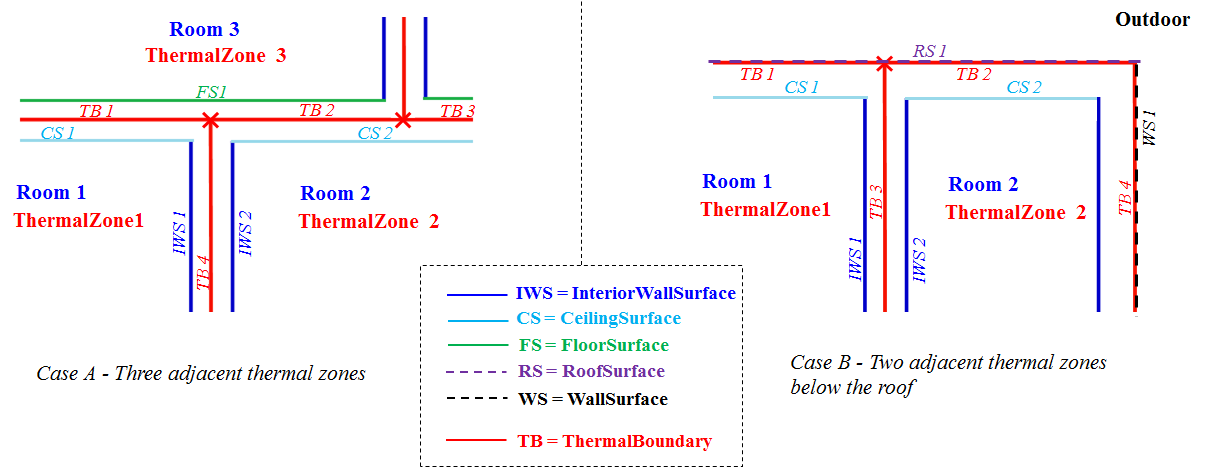
\includegraphics{fig/ThermalZoneAdjacency.png}
\caption{Schema of adjacent thermal zones}
\end{figure}

\texttt{ThermalBoundary} may contain attributes characterizing their
type\\
(\texttt{thermalBoundaryType}), orientation (\texttt{azimuth} and
\texttt{inclination}) and explicit geometry (\texttt{surfaceGeometry}).
All these attributes are optional. Thus, a \texttt{ThermalZone} may
optionally contain an explicit surface geometry (specified by
\texttt{surfaceGeometry}), useful in particular for visualisation
purposes if the \texttt{ThermalBoundary} does not coincide with any
\texttt{\_BoundarySurface}, but not necessary for heating and cooling
demand calculations.

The \texttt{ThermalBoundaryType} type is slightly different to the types
of \texttt{\_BoundarySurface} from CityGML, integrating further thermal
boundaries like AtticFloor, BasementCeiling, BasementFloor or
SharedWall.

Each \texttt{ThermalBoundaryType} is composed of
\texttt{ThermalComponent} (e.g.~wall construction, windows etc.) which
holds the \texttt{Construction}.

In the following, two XML examples of \texttt{ThermalBoundary}, with and
without explicit geometry are given.

\begin{Shaded}
\begin{Highlighting}[]
\CommentTok{<!--Example of a ThermalBoundary corresponding to a building roof, delimiting a thermal zone -->}
\KeywordTok{<energy:ThermalBoundary}\OtherTok{ gml:id=}\StringTok{"id_thermalboundary_1"}\KeywordTok{>}
    \KeywordTok{<gml:description>}\NormalTok{Thermal Boundary 1}\KeywordTok{</gml:description>}
    \KeywordTok{<gml:name>}\NormalTok{Thermal Boundary 1}\KeywordTok{</gml:name>}
    \KeywordTok{<energy:azimuth}\OtherTok{ uom=}\StringTok{"decimal degrees"}\KeywordTok{>}\NormalTok{135}\KeywordTok{</energy:azimuth>}
    \KeywordTok{<energy:inclination}\OtherTok{ uom=}\StringTok{"decimal degrees"}\KeywordTok{>}\NormalTok{55}\KeywordTok{</energy:inclination>}
    \KeywordTok{<energy:thermalBoundaryType>}\NormalTok{Roof}\KeywordTok{</energy:thermalBoundaryType>}
    \KeywordTok{<partOf}\OtherTok{ xlink:href=}\StringTok{"#id_thermalzone_1"}\KeywordTok{/>}
    \KeywordTok{<energy:composedOf>}
        \KeywordTok{<energy:ThermalComponent}\OtherTok{ gml:id=}\StringTok{"id_thermalcomponent_1"}\KeywordTok{>}
            \CommentTok{<!--Here come all attributes of the first ThermalComponent (omitted here)-->}
        \KeywordTok{</energy:ThermalComponent>}
    \KeywordTok{</energy:composedOf>}
    \KeywordTok{<energy:composedOf>}
        \KeywordTok{<energy:ThermalComponent}\OtherTok{ gml:id=}\StringTok{"id_thermalcomponent_2"}\KeywordTok{>}
            \CommentTok{<!--Here come all attributes of the second ThermalComponent (omitted here)-->}
        \KeywordTok{</energy:ThermalComponent>}
    \KeywordTok{</energy:composedOf>}
    \KeywordTok{<correspondsTo}\OtherTok{ xlink:href=}\StringTok{"#id_RoofSurface_1"}\KeywordTok{/>}
\KeywordTok{</energy:ThermalBoundary>}
\end{Highlighting}
\end{Shaded}

\begin{Shaded}
\begin{Highlighting}[]
\CommentTok{<!--Example of a ThermalBoundary with explicit surface geometry, separating two thermal zones -->}
\KeywordTok{<energy:ThermalBoundary}\OtherTok{ gml:id=}\StringTok{"id_thermalboundary_2"}\KeywordTok{>}
    \CommentTok{<!--Additional attributes of the ThermalBoundary class (omitted here)-->}

    \KeywordTok{<energy:surfaceGeometry>}
        \KeywordTok{<gml:MultiSurface}\OtherTok{ gml:id=}\StringTok{"id_thermalboundary_2_surface_geometry"}\OtherTok{ srsName=}\StringTok{"EPSG:31256"}\OtherTok{ srsDimension=}\StringTok{"3"}\KeywordTok{>}
            \KeywordTok{<gml:surfaceMember>}
                \KeywordTok{<gml:Polygon>}
                    \KeywordTok{<gml:exterior>}
                        \KeywordTok{<gml:LinearRing>}
                            \KeywordTok{<gml:posList>}\NormalTok{0 0 0 0 10 0 5 10 0 5 0 0 0 0 0}\KeywordTok{</gml:posList>}
                        \KeywordTok{</gml:LinearRing>}
                    \KeywordTok{</gml:exterior>}
                \KeywordTok{</gml:Polygon>}
            \KeywordTok{</gml:surfaceMember>}
        \KeywordTok{</gml:MultiSurface>}
    \KeywordTok{</energy:surfaceGeometry>}
    \KeywordTok{<partOf}\OtherTok{ xlink:href=}\StringTok{"#id_thermalzone_1"}\KeywordTok{/>}
    \KeywordTok{<partOf}\OtherTok{ xlink:href=}\StringTok{"#id_thermalzone_2"}\KeywordTok{/>}
\KeywordTok{</energy:ThermalBoundary>}
\end{Highlighting}
\end{Shaded}

\subsubsection{ThermalComponent}\label{thermalcomponent}

A \texttt{ThermalComponent} object is a part of the thermal boundary
corresponding to a homogeneous construction component (e.g.~windows,
wall, insulated part of a wall etc.). Each \texttt{ThermalComponent} is
characterized with their \texttt{Area}, information whether it is
coupled to ground (\texttt{isGroundCoupled}) and exposed to sun
(\texttt{isSunExposed}).

Since \texttt{ThermalComponent} inherits from \texttt{\_CityObject}, it
can be associated to a \texttt{Construction} object (see module
Construction and Material). This may be done either inline or by means
of xlinks (see example below). In this way, \texttt{ThermalComponent}
provides the physical properties of the building envelope to calculate
the heating and cooling demand.

\begin{Shaded}
\begin{Highlighting}[]
\CommentTok{<!--Example of a ThermalComponent-->}
\KeywordTok{<energy:ThermalComponent}\OtherTok{ gml:id=}\StringTok{"id_thermalcomponent_1"}\KeywordTok{>}
    \KeywordTok{<gml:description>}\NormalTok{Thermal Component 1}\KeywordTok{</gml:description>}
    \KeywordTok{<gml:name>}\NormalTok{Thermal Component 1}\KeywordTok{</gml:name>}
    \KeywordTok{<energy:construction}\OtherTok{ xlink:href=}\StringTok{"#id_construction_1"}\KeywordTok{/>}
    \KeywordTok{<energy:area}\OtherTok{ uom=}\StringTok{"m^2"}\KeywordTok{>}\NormalTok{50.0}\KeywordTok{</energy:area>}
    \KeywordTok{<energy:isGroundCoupled>}\NormalTok{false}\KeywordTok{</energy:isGroundCoupled>}
    \KeywordTok{<energy:isSunExposed>}\NormalTok{true}\KeywordTok{</energy:isSunExposed>}
\KeywordTok{</energy:ThermalComponent>}
\end{Highlighting}
\end{Shaded}

\section{Temporal Data Module}\label{temporal-data-module}

\subsection{Time Series}\label{time-series}

\begin{figure}[htbp]
\centering
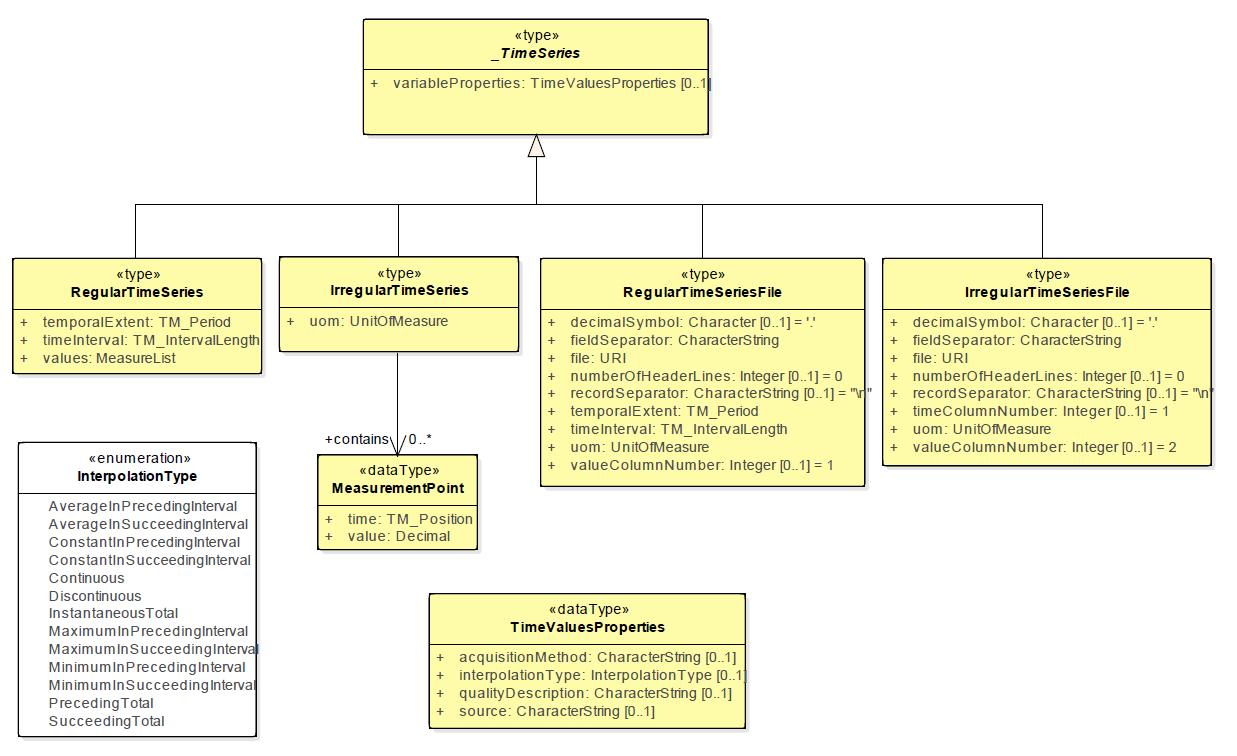
\includegraphics{fig/class_time.png}
\caption{Class diagram of ADE Energy Core - Time Series}
\end{figure}

Time series are homogeneous lists of time-depending values. They are
used in the Energy ADE to store energy amount or a schedule, for
instance. As they actually are a data type which is not domain-specific,
they are planned to be integrated in the CityGML 3.0. All time series
share some common properties, contained in the variableProperties
attribute. These properties are the variable label, the variable unit of
measure (\emph{uom}), the interpolation type (based on the
\href{http://def.seegrid.csiro.au/sissvoc/ogc-def/resource?uri=http://www.opengis.net/def/waterml/2.0/interpolationType/}{WaterML
ADE} and some further metadata like the data source, the acquisition
method and a quality description.

Time series can be either regular or irregular. \emph{RegularTimeSeries}
contain values generated at regularly spaced interval of time
(\texttt{timeInterval}), over a given \texttt{temporalExtent}
(i.e.~start, end and duration time). They are used, for instance, to
store automatically acquired data or hourly/daily/monthly simulation
results. In \emph{IrregularTimeSeries}, data follows a temporal
sequence, but the measurement points may not happen at a regular time
interval
(\href{http://www-01.ibm.com/support/knowledgecenter/SSCRJU_3.0.0/com.ibm.swg.im.infosphere.streams.timeseries-toolkit.doc/doc/timeseries-regular.html}{IBM
knowledge Center}). Therefore, each value must be associated with a data
or time. What is more, each time series can be stored as an external
file (e.g.~csv or text) and for this purpose a number of attributes
provide the required information about how to retrieve the proper set of
values from the files. In the following, several examples of time series
are given. Please note that the variableProperties are presented in the
first example and omitted in the following ones for better readability.

\begin{Shaded}
\begin{Highlighting}[]
\CommentTok{<!--Example of RegularTimeSeries object with 12 monthly values-->}
\KeywordTok{<energy:RegularTimeSeries}\OtherTok{ gml:id=}\StringTok{"id_timeseries_electricity_demand_1"}\KeywordTok{>}
    \KeywordTok{<energy:variableProperties>}
        \KeywordTok{<energy:TimeValuesProperties>}
            \KeywordTok{<energy:acquisitionMethod>}\NormalTok{Description of the acquisition method}\KeywordTok{</energy:acquisitionMethod>}
            \KeywordTok{<energy:interpolationType>}\NormalTok{AverageInSucceedingInterval}\KeywordTok{</energy:interpolationType>}
            \KeywordTok{<energy:qualityDescription>}\NormalTok{Description of data quality}\KeywordTok{</energy:qualityDescription>}
            \KeywordTok{<energy:source>}\NormalTok{Information about data source}\KeywordTok{</energy:source>}
        \KeywordTok{</energy:TimeValuesProperties>}
    \KeywordTok{</energy:variableProperties>}
    \KeywordTok{<energy:temporalExtent>}
        \KeywordTok{<gml:TimePeriod>}
            \KeywordTok{<gml:beginPosition>}\NormalTok{2016-01-01}\KeywordTok{</gml:beginPosition>}
            \KeywordTok{<gml:endPosition>}\NormalTok{2016-12-31}\KeywordTok{</gml:endPosition>}
        \KeywordTok{</gml:TimePeriod>}
    \KeywordTok{</energy:temporalExtent>}
    \KeywordTok{<energy:timeInterval}\OtherTok{ unit=}\StringTok{"year"}\KeywordTok{>}\NormalTok{0.0833}\KeywordTok{</energy:timeInterval>}
    \KeywordTok{<energy:values}\OtherTok{ uom=}\StringTok{"kWh"}\KeywordTok{>}\NormalTok{330 320 300 270 200 180 160 155 170 200 250 300}\KeywordTok{</energy:values>}
\KeywordTok{</energy:RegularTimeSeries>}
\end{Highlighting}
\end{Shaded}

\begin{Shaded}
\begin{Highlighting}[]
\CommentTok{<!--Example of RegularTimeSeries object with daily values (exerpt)-->}
\KeywordTok{<energy:RegularTimeSeries}\OtherTok{ gml:id=}\StringTok{"id_timeseries_electricity_demand_2"}\KeywordTok{>}
    \KeywordTok{<energy:temporalExtent>}
        \KeywordTok{<gml:TimePeriod>}
            \KeywordTok{<gml:beginPosition>}\NormalTok{2011-01-01}\KeywordTok{</gml:beginPosition>}
            \KeywordTok{<gml:endPosition>}\NormalTok{2011-12-31}\KeywordTok{</gml:endPosition>}
        \KeywordTok{</gml:TimePeriod>}
    \KeywordTok{</energy:temporalExtent>}
    \KeywordTok{<energy:timeInterval}\OtherTok{ unit=}\StringTok{"day"}\KeywordTok{>}\NormalTok{1}\KeywordTok{</energy:timeInterval>}
    \KeywordTok{<energy:values}\OtherTok{ uom=}\StringTok{"kWh"}\KeywordTok{>}\NormalTok{11.2 11.4 10.2 9.6 6.3 11.5 12.7 ... (truncated, set of 365 values) }\KeywordTok{</energy:values>}
\KeywordTok{</energy:RegularTimeSeries>}
\end{Highlighting}
\end{Shaded}

\begin{Shaded}
\begin{Highlighting}[]
\CommentTok{<!--Example of RegularTimeSeriesFile object with hourly values contained in a file-->}
\KeywordTok{<energy:RegularTimeSeriesFile}\OtherTok{ gml:id=}\StringTok{"id_regulartimeseries_file_1"}\KeywordTok{>}
    \KeywordTok{<energy:uom}\OtherTok{ uom=}\StringTok{"W/m^2"}\KeywordTok{/>}
    \KeywordTok{<energy:file>}\NormalTok{file_name_containing_values.tsv}\KeywordTok{</energy:file>}
    \KeywordTok{<energy:temporalExtent>}
    \KeywordTok{<energy:temporalExtent>}
        \KeywordTok{<gml:TimePeriod>}
            \KeywordTok{<gml:beginPosition>}\NormalTok{2008-01-01}\KeywordTok{</gml:beginPosition>}
            \KeywordTok{<gml:endPosition>}\NormalTok{2008-12-31}\KeywordTok{</gml:endPosition>}
        \KeywordTok{</gml:TimePeriod>}
    \KeywordTok{</energy:temporalExtent>}
    \KeywordTok{<energy:timeInterval}\OtherTok{ unit=}\StringTok{"hour"}\KeywordTok{>}\NormalTok{1}\KeywordTok{</energy:timeInterval>}
    \KeywordTok{<energy:numberOfHeaderLines>}\NormalTok{1}\KeywordTok{</energy:numberOfHeaderLines>}
    \KeywordTok{<energy:valueColumnNumber>}\NormalTok{1}\KeywordTok{</energy:valueColumnNumber>}
    \KeywordTok{<energy:fieldSeparator>}\NormalTok{\textbackslash{}t}\KeywordTok{</energy:fieldSeparator>}
\KeywordTok{</energy:RegularTimeSeriesFile>}
\end{Highlighting}
\end{Shaded}

\begin{Shaded}
\begin{Highlighting}[]
\CommentTok{<!--Example of IrregularTimeSeries object-->}
\end{Highlighting}
\end{Shaded}

\subsection{Schedules}\label{schedules}

\begin{figure}[htbp]
\centering
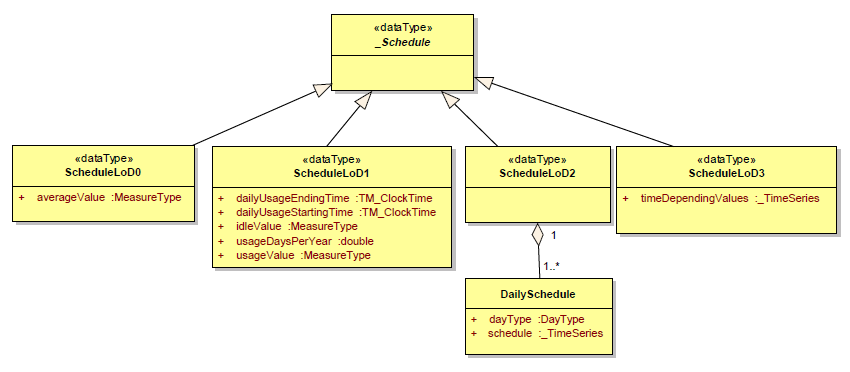
\includegraphics{fig/class_schedules.png}
\caption{Class diagram of ADE Energy Core - Schedules}
\end{figure}

The type Schedule is used in the Energy ADE for different kinds of
schedules, e.g.~heating/cooling schedules (set-point temperatures),
ventilation schedules (mechanical air change rate) and occupancy rate.
Schedules can be modelled up to 4 ``semantic'' levels of details
depending on the available information and the application requirement.
These levels of detail range from a simple constant value to a schedule
characterised by a \_TimeSeries object.

\subsubsection{ConstantValueSchedule}\label{constantvalueschedule}

The simplest level of detail, this Schedule is defined by a constant
value, generally corresponding to the average parameter value.

\begin{Shaded}
\begin{Highlighting}[]
\CommentTok{<!--Example of a ConstantValueSchedule-->}
\KeywordTok{<energy:ConstantValueSchedule}\OtherTok{ gml:id=}\StringTok{"id_constant_schedule_1"}\KeywordTok{>}
    \KeywordTok{<energy:averageValue}\OtherTok{ uom=}\StringTok{"degree Celsius"}\KeywordTok{>}\NormalTok{26}\KeywordTok{</energy:averageValue>}
\KeywordTok{</energy:ConstantValueSchedule>}
\end{Highlighting}
\end{Shaded}

\subsubsection{DualValueSchedule}\label{dualvalueschedule}

A two-state schedule, this schedule is defined by a usage value for
usage times, and an idle value outside this temporal boundaries.
Information about the number of usage days per year and usage hours per
usage days are also defined. This schedule complies in particular with
the data requirements of the codes and norms describing the monthly
energy balance (DIN 18599-2, ISO 13790).

\begin{Shaded}
\begin{Highlighting}[]
\CommentTok{<!--Example of a DualValueSchedule-->}
\KeywordTok{<energy:DualValueSchedule}\OtherTok{ gml:id=}\StringTok{"id_dualvalue_schedule_2"}\KeywordTok{>}
    \KeywordTok{<energy:usageValue}\OtherTok{ uom=}\StringTok{"degree Celsius"}\KeywordTok{>}\NormalTok{20}\KeywordTok{</energy:usageValue>}
    \KeywordTok{<energy:idleValue}\OtherTok{ uom=}\StringTok{"degree Celsius"}\KeywordTok{>}\NormalTok{16}\KeywordTok{</energy:idleValue>}
    \KeywordTok{<energy:usageHoursPerDay}\OtherTok{ uom=}\StringTok{"hour"}\KeywordTok{>}\NormalTok{17}\KeywordTok{</energy:usageHoursPerDay>}
    \KeywordTok{<energy:usageDaysPerYear}\OtherTok{ uom=}\StringTok{"day"}\KeywordTok{>}\NormalTok{365}\KeywordTok{</energy:usageDaysPerYeary>}
\KeywordTok{</energy:DualValueSchedule>}
\end{Highlighting}
\end{Shaded}

\subsubsection{DailyPatternSchedule}\label{dailypatternschedule}

Detailed schedule composed of daily schedules associated to recurrent
day types (weekday, weekend etc.). These daily schedules are Time Series
as described above.

\begin{Shaded}
\begin{Highlighting}[]
\CommentTok{<!--Example of a daily pattern schedule for a standard day-->}
\KeywordTok{<energy:DailyPatternSchedule}\OtherTok{ gml:id=}\StringTok{"id_dailypattern_schedule_3"}\KeywordTok{>}
    \KeywordTok{<energy:dailySchedule>}
        \KeywordTok{<energy:DailySchedule>}
            \KeywordTok{<energy:dayType>}\NormalTok{CustomDay1}\KeywordTok{</energy:dayType>}
            \KeywordTok{<energy:schedule>}
                \KeywordTok{<energy:RegularTimeSeries}\OtherTok{ gml:id=}\StringTok{"id_occupants_daily_timeseries_1"}\KeywordTok{>}
                    \KeywordTok{<energy:temporalExtent>}
                        \KeywordTok{<gml:TimePeriod>}
                            \KeywordTok{<gml:beginPosition>}\NormalTok{00:00:00}\KeywordTok{</gml:beginPosition>}
                            \KeywordTok{<gml:endPosition>}\NormalTok{23:59:59}\KeywordTok{</gml:endPosition>}
                        \KeywordTok{</gml:TimePeriod>}
                    \KeywordTok{</energy:temporalExtent>}
                    \KeywordTok{<energy:timeInterval}\OtherTok{ unit=}\StringTok{"hour"}\KeywordTok{>}\NormalTok{1}\KeywordTok{</energy:timeInterval>}
                    \KeywordTok{<energy:values}\OtherTok{ uom=}\StringTok{"ratio"}\KeywordTok{>}\NormalTok{1 1 1 0.74 0.35 ... (truncated, set of 24 values)}\KeywordTok{</energy:values>}
                \KeywordTok{</energy:RegularTimeSeries>}
            \KeywordTok{</energy:schedule>}
        \KeywordTok{</energy:DailySchedule>}
    \KeywordTok{</energy:dailySchedule>}
\KeywordTok{</energy:DailyPatternSchedule>}
\end{Highlighting}
\end{Shaded}

\begin{Shaded}
\begin{Highlighting}[]
\CommentTok{<!--Example of a daily pattern schedule for a standard week composed of weekday and weekend days-->}
\KeywordTok{<energy:DailyPatternSchedule}\OtherTok{ gml:id=}\StringTok{"id_dailypattern_schedule_4"}\KeywordTok{>}
    \KeywordTok{<energy:dailySchedule>}
        \KeywordTok{<energy:DailySchedule>}
            \KeywordTok{<energy:dayType>}\NormalTok{WeekDay}\KeywordTok{</energy:dayType>}
            \KeywordTok{<energy:schedule>}
                \KeywordTok{<energy:RegularTimeSeries}\OtherTok{ gml:id=}\StringTok{"id_occupants_daily_timeseries_2"}\KeywordTok{>}
                    \KeywordTok{<energy:temporalExtent>}
                        \KeywordTok{<gml:TimePeriod>}
                            \KeywordTok{<gml:beginPosition>}\NormalTok{00:00:00}\KeywordTok{</gml:beginPosition>}
                            \KeywordTok{<gml:endPosition>}\NormalTok{23:59:59}\KeywordTok{</gml:endPosition>}
                        \KeywordTok{</gml:TimePeriod>}
                    \KeywordTok{</energy:temporalExtent>}
                    \KeywordTok{<energy:timeInterval}\OtherTok{ unit=}\StringTok{"hour"}\KeywordTok{>}\NormalTok{1}\KeywordTok{</energy:timeInterval>}
                    \KeywordTok{<energy:values}\OtherTok{ uom=}\StringTok{"ratio"}\KeywordTok{>}\NormalTok{0 0 0 0.1 0.2 0.5 ... (truncated, set of 24 values)}\KeywordTok{</energy:values>}
                \KeywordTok{</energy:RegularTimeSeries>}
            \KeywordTok{</energy:schedule>}
        \KeywordTok{</energy:DailySchedule>}
    \KeywordTok{</energy:dailySchedule>}
    \KeywordTok{<energy:dailySchedule>}
        \KeywordTok{<energy:DailySchedule>}
            \KeywordTok{<energy:dayType>}\NormalTok{WeenEnd}\KeywordTok{</energy:dayType>}
            \KeywordTok{<energy:schedule>}
                \KeywordTok{<energy:RegularTimeSeries}\OtherTok{ gml:id=}\StringTok{"id_occupants_daily_timeseries_3"}\KeywordTok{>}
                    \KeywordTok{<energy:temporalExtent>}
                        \KeywordTok{<gml:TimePeriod>}
                            \KeywordTok{<gml:beginPosition>}\NormalTok{00:00:00}\KeywordTok{</gml:beginPosition>}
                            \KeywordTok{<gml:endPosition>}\NormalTok{23:59:59}\KeywordTok{</gml:endPosition>}
                        \KeywordTok{</gml:TimePeriod>}
                    \KeywordTok{</energy:temporalExtent>}
                    \KeywordTok{<energy:timeInterval}\OtherTok{ unit=}\StringTok{"hour"}\KeywordTok{>}\NormalTok{1}\KeywordTok{</energy:timeInterval>}
                    \KeywordTok{<energy:values}\OtherTok{ uom=}\StringTok{"ratio"}\KeywordTok{>}\NormalTok{0 0 0 0.11 0.22 ... (truncated, set of 24 values)}\KeywordTok{</energy:values>}
                \KeywordTok{</energy:RegularTimeSeries>}
            \KeywordTok{</energy:schedule>}
        \KeywordTok{</energy:DailySchedule>}
    \KeywordTok{</energy:dailySchedule>}
\KeywordTok{</energy:DailyPatternSchedule>}
\end{Highlighting}
\end{Shaded}

\subsubsection{TimeSeriesSchedule}\label{timeseriesschedule}

Most detailed schedule corresponding to a Time series as described
above.

\begin{Shaded}
\begin{Highlighting}[]
\CommentTok{<!--Example of a time series based schedule with hourly values for one year-->}
\KeywordTok{<energy:TimeSeriesSchedule}\OtherTok{ gml:id=}\StringTok{"id_timeseries_schedule_5"}\KeywordTok{>}
    \KeywordTok{<energy:RegularTimeSeries} \ErrorTok{"id_occupants_timeseries_5"}\KeywordTok{>}
            \KeywordTok{<energy:temporalExtent>}
                \KeywordTok{<gml:TimePeriod>}
                    \KeywordTok{<gml:beginPosition>}\NormalTok{2000-01-01}\KeywordTok{</gml:beginPosition>}
                    \KeywordTok{<gml:endPosition>}\NormalTok{2000-12-31}\KeywordTok{</gml:endPosition>}
                \KeywordTok{</gml:TimePeriod>}
            \KeywordTok{</energy:temporalExtent>}
            \KeywordTok{<energy:timeInterval}\OtherTok{ unit=}\StringTok{"hour"}\KeywordTok{>}\NormalTok{1}\KeywordTok{</energy:timeInterval>}
            \KeywordTok{<energy:values}\OtherTok{ uom=}\StringTok{"ratio"}\KeywordTok{>}\NormalTok{1 1 1 1 0.9 0.7 0.5 ... (truncated, set of 8760 values)}\KeywordTok{</energy:values>}
    \KeywordTok{</energy:RegularTimeSeries>}
\KeywordTok{</energy:TimeSeriesSchedule>}
\end{Highlighting}
\end{Shaded}

\section{Construction and Material
Module}\label{construction-and-material-module}

\begin{figure}[htbp]
\centering
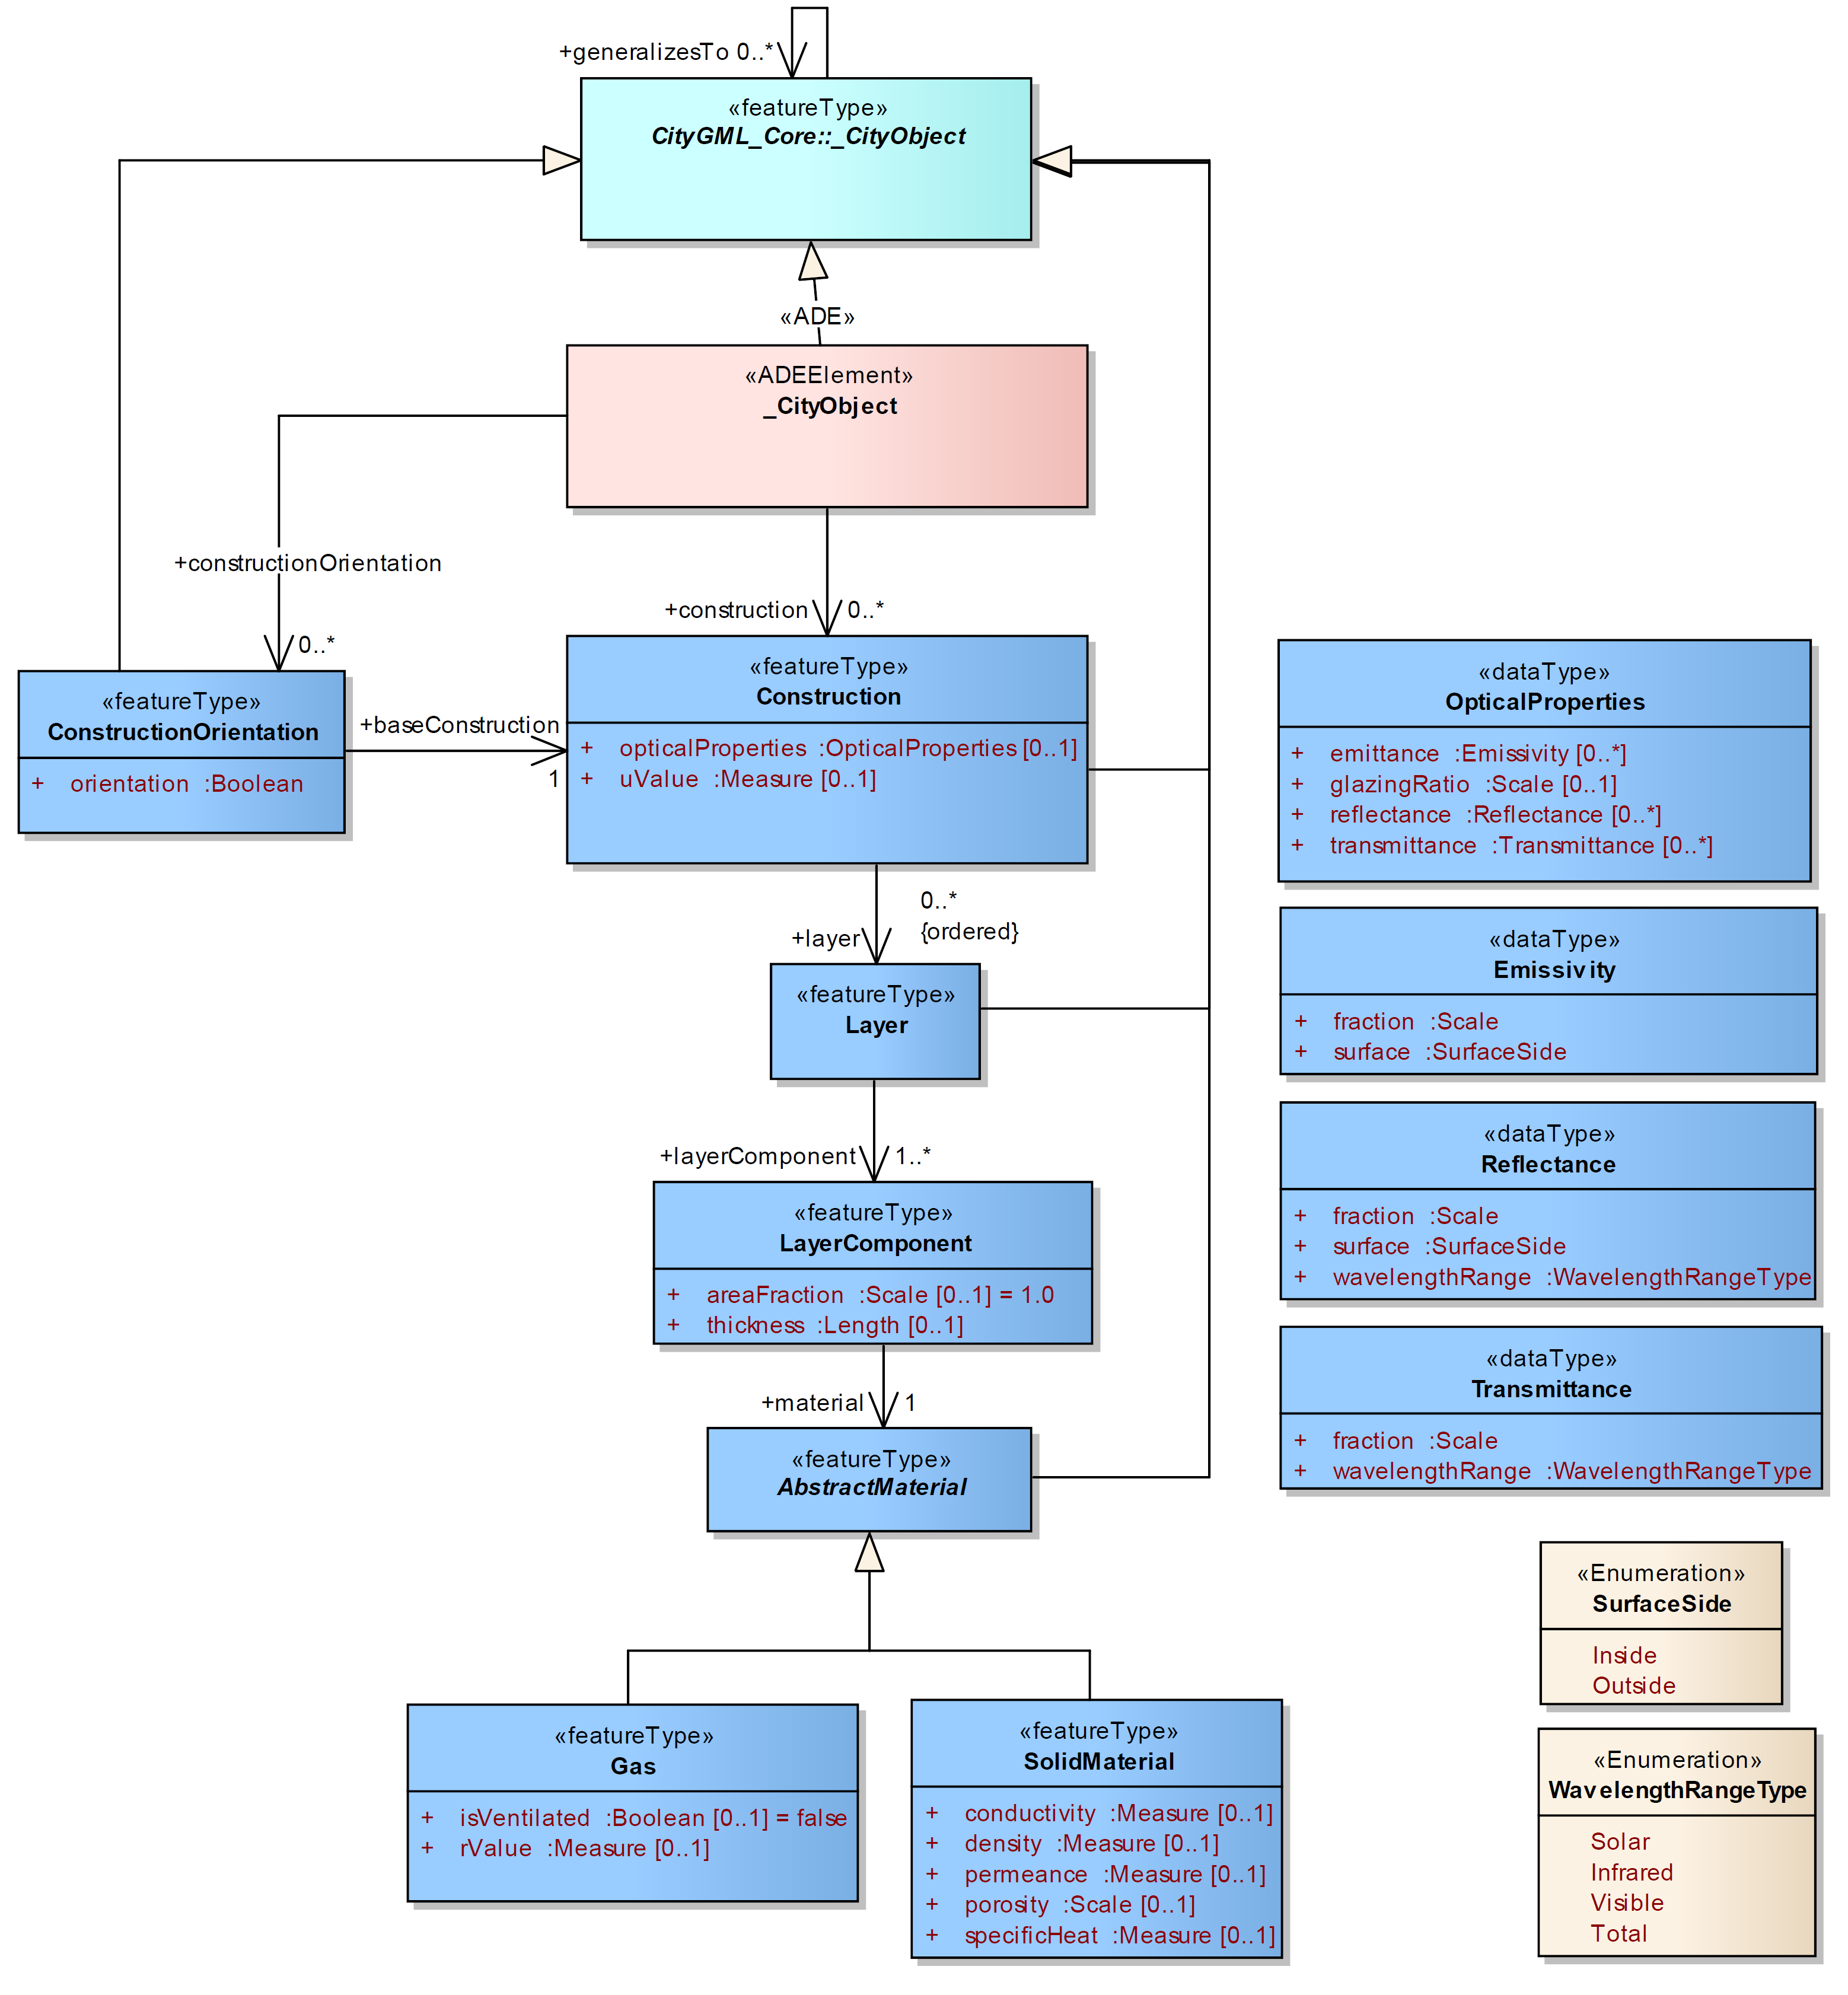
\includegraphics{fig/class_construction.png}
\caption{Class diagram of Construction Module}
\end{figure}

The Construction and Material module of the ADE Energy contains the
physical characterization of the boundary surfaces, surface components
and, possibly, even the whole building. As it inherits from class
\texttt{\_CityObject}, all similar objects can be described also by
means of construction and materials. Given that the nature of this
module is not domain-specific, it can be used beyond energy-related
applications (e.g.~in statics, acoustics etc.).

\subsection{Construction}\label{construction}

Physical characterisation of building envelop or intern room partition
(e.g.~wall, roof, openings), it may be specified as an ordered
combination of layers. In the Energy ADE, the object Construction can be
linked to the \texttt{\_ThermalComponents}, in order to defined the
physical parameters of a walls, roofs of windows, for a space
heating/cooling calculation. However, it may possibly be linked to any
\texttt{\_CityObject} for other purposes, in particular to
\texttt{\_BoundarySurface}, \texttt{\_Opening} or even
\texttt{\_AbstractBuilding}. Each construction object is characterised
by a number of attributes like the U-value, or some optical properties,
like transmittance, reflecatance and emissivity. In particular,
\emph{Transmittance} is the fraction of incident radiation which passes
through a specific object. It is specified for a given wavelength range
type (\texttt{wavelengthRange}). For example, the total transmittance of
a window correspond to its \emph{g-value} (also called Solar Heat Gain
Coefficient). The transmittance value is included between 0 (completely
opaque object) and 1 (completely transparent object). \emph{Reflectance}
is the fraction of incident radiation which is reflected by an object.
It is specified for a given surface (\texttt{SurfaceSide}) and for a
given wavelength range type. \emph{Emissivity} is the ratio of the
infrared (also called long-wave) radiation emitted by a specific
surface/object to that of a black body. It is specified for a given
surface (SurfaceSide). According with the Kirchoff and Lambert law, for
a diffuse grey body the aborptance and the emittance are equal for a
given wavelength range. The sum of the transmittance, reflectance and
emissivity (or absorptance) fractions of a surface/object is always 1.
In the following, several examples of Construction objects are
presented, with different levels of complexity.

\begin{Shaded}
\begin{Highlighting}[]
\CommentTok{<!--Example of Construction object-->}
\end{Highlighting}
\end{Shaded}

\begin{Shaded}
\begin{Highlighting}[]
\CommentTok{<!--Example of a simple wall construction just with a U-value-->}
\KeywordTok{<energy:Construction}\OtherTok{ gml:id=}\StringTok{"id_construction_2"}\KeywordTok{>}
    \KeywordTok{<gml:description>}\NormalTok{Description of Construction 2}\KeywordTok{</gml:description>}
    \KeywordTok{<gml:name>}\NormalTok{Name of Construction 2}\KeywordTok{</gml:name>}
    \KeywordTok{<energy:uValue}\OtherTok{ uom=}\StringTok{"W/(K*m^2)"}\KeywordTok{>}\NormalTok{3.0}\KeywordTok{</energy:uValue>}
\KeywordTok{</energy:Construction>}
\end{Highlighting}
\end{Shaded}

\begin{Shaded}
\begin{Highlighting}[]
\CommentTok{<!--Example of window Construction object-->}
\KeywordTok{<energy:Construction}\OtherTok{ gml:id=}\StringTok{"id_construction_2"}\KeywordTok{>}
    \KeywordTok{<gml:description>}\NormalTok{Description of the windows Construction}\KeywordTok{</gml:description>}
    \KeywordTok{<gml:name>}\NormalTok{Name of the window Construction}\KeywordTok{</gml:name>}

    \KeywordTok{<energy:uValue}\OtherTok{ uom=}\StringTok{"W/(K*m^2)"}\KeywordTok{>}\NormalTok{1.9}\KeywordTok{</energy:uValue>}
    \KeywordTok{<energy:opticalProperties>}
        \KeywordTok{<energy:OpticalProperties>}
            \KeywordTok{<energy:emittance>}
                \KeywordTok{<energy:Emissivity>}
                    \KeywordTok{<energy:fraction}\OtherTok{ uom=}\StringTok{"ratio"}\KeywordTok{>}\NormalTok{0.1}\KeywordTok{</energy:fraction>}
                    \KeywordTok{<energy:surface>}\NormalTok{Outside}\KeywordTok{</energy:surface>}
                \KeywordTok{</energy:Emissivity>}
            \KeywordTok{</energy:emittance>}
            \KeywordTok{<energy:reflectance>}
                \KeywordTok{<energy:Reflectance>}
                    \KeywordTok{<energy:fraction}\OtherTok{ uom=}\StringTok{"ratio"}\KeywordTok{>}\NormalTok{0.1}\KeywordTok{</energy:fraction>}
                    \KeywordTok{<energy:surface>}\NormalTok{Outside}\KeywordTok{</energy:surface>}
                    \KeywordTok{<energy:wavelengthRange>}\NormalTok{Solar}\KeywordTok{</energy:wavelengthRange>}
                \KeywordTok{</energy:Reflectance>}
            \KeywordTok{</energy:reflectance>}
            \KeywordTok{<energy:transmittance>}
                \KeywordTok{<energy:Transmittance>}
                    \KeywordTok{<energy:fraction}\OtherTok{ uom=}\StringTok{"ratio"}\KeywordTok{>}\NormalTok{0.8}\KeywordTok{</energy:fraction>}
                    \KeywordTok{<energy:wavelengthRange>}\NormalTok{Solar}\KeywordTok{</energy:wavelengthRange>}
                \KeywordTok{</energy:Transmittance>}
            \KeywordTok{</energy:transmittance>}
            \KeywordTok{<energy:glazingRatio}\OtherTok{ uom=}\StringTok{"ratio"}\KeywordTok{>}\NormalTok{0.9}\KeywordTok{</energy:glazingRatio>}
        \KeywordTok{</energy:OpticalProperties>}
    \KeywordTok{</energy:opticalProperties>}

\KeywordTok{</energy:Construction>}
\end{Highlighting}
\end{Shaded}

\subsection{ConstructionOrientation}\label{constructionorientation}

This class defines the orientation convention of the
\texttt{Construction} object it is referred to. In other words, it
indicates in which order the layers are to be considered (from inside to
outside, or viceversa), because the same construction, if common to
different zones or buildings, might be orientated in two different
directions for instance.

\begin{Shaded}
\begin{Highlighting}[]
\CommentTok{<!--Example of ConstructionOrientation object-->}
\KeywordTok{<energy:ConstructionOrientation}\OtherTok{ gml:id=}\StringTok{"id_construction_orientation_ground_1"}\KeywordTok{>}
    \KeywordTok{<gml:description>}\NormalTok{Description of Construction Orientation 1 (from inside to outside)}\KeywordTok{</gml:description>}
    \KeywordTok{<gml:name>}\NormalTok{Name of Construction Orientation 1}\KeywordTok{</gml:name>}
    \KeywordTok{<energy:orientation>}\NormalTok{true}\KeywordTok{</energy:orientation>}
    \KeywordTok{<energy:baseConstruction}\OtherTok{ xlink:href=}\StringTok{"#id_construction_1"}\KeywordTok{/>}
\KeywordTok{</energy:ConstructionOrientation>}
\end{Highlighting}
\end{Shaded}

\subsubsection{Layer}\label{layer}

Combination of one of more materials, referenced via a layer component.
It inherits from \texttt{\_CityObject}.

\subsubsection{LayerComponent}\label{layercomponent}

Homogeneous part of a layer, covering a given fraction
(\texttt{areaFraction}) of the layer.

\subsection{Materials}\label{materials}

\subsubsection{AbstractMaterial}\label{abstractmaterial}

Abstract superclass for all Material classes. A Material is a
homogeneous substance. We distinguish solid materials (with mass) from
gas (without mass).

\subsubsection{SolidMaterial}\label{solidmaterial}

Class of the materials which have a mass and a heat capacity.

\begin{Shaded}
\begin{Highlighting}[]
\CommentTok{<!--Example of a three layered construction-->}
\KeywordTok{<energy:Construction}\OtherTok{ gml:id=}\StringTok{"ThreeLayeredMaterial"}\KeywordTok{>}
    \KeywordTok{<energy:layer>}
        \KeywordTok{<energy:Layer>}
            \KeywordTok{<energy:layerComponent>}
                \KeywordTok{<energy:LayerComponent>}
                    \KeywordTok{<energy:thickness}\OtherTok{ uom=}\StringTok{"m"}\KeywordTok{>}\NormalTok{0.24}\KeywordTok{</energy:thickness>}
                    \KeywordTok{<energy:material>}
                        \KeywordTok{<energy:SolidMaterial>}
                            \KeywordTok{<gml:name>}\NormalTok{Concrete 2100}\KeywordTok{</gml:name>}
                            \KeywordTok{<energy:conductivity}\OtherTok{ uom=}\StringTok{"W/(K*m^2)"}\KeywordTok{>}\NormalTok{2.035}\KeywordTok{</energy:conductivity>}
                            \KeywordTok{<energy:density}\OtherTok{ uom=}\StringTok{"kg/m^3"}\KeywordTok{>}\NormalTok{2100.0}\KeywordTok{</energy:density>}
                            \KeywordTok{<energy:specificHeat}\OtherTok{ uom=}\StringTok{"J/(K*kg)"}\KeywordTok{>}\NormalTok{920.0}\KeywordTok{</energy:specificHeat>}
                        \KeywordTok{</energy:SolidMaterial>}
                    \KeywordTok{</energy:material>}
                \KeywordTok{</energy:LayerComponent>}
            \KeywordTok{</energy:layerComponent>}

            \KeywordTok{<energy:layerComponent>}
                \KeywordTok{<energy:LayerComponent>}
                    \KeywordTok{<energy:thickness}\OtherTok{ uom=}\StringTok{"m"}\KeywordTok{>}\NormalTok{0.062}\KeywordTok{</energy:thickness>}
                    \KeywordTok{<energy:material>}
                        \KeywordTok{<energy:SolidMaterial>}
                            \KeywordTok{<gml:name>}\NormalTok{Insulation 047}\KeywordTok{</gml:name>}
                            \KeywordTok{<energy:conductivity}\OtherTok{ uom=}\StringTok{"W/(K*m^2)"}\KeywordTok{>}\NormalTok{0.047}\KeywordTok{</energy:conductivity>}
                            \KeywordTok{<energy:density}\OtherTok{ uom=}\StringTok{"kg/m^3"}\KeywordTok{>}\NormalTok{75.0}\KeywordTok{</energy:density>}
                            \KeywordTok{<energy:specificHeat}\OtherTok{ uom=}\StringTok{"J/(K*kg)"}\KeywordTok{>}\NormalTok{840.0}\KeywordTok{</energy:specificHeat>}
                        \KeywordTok{</energy:SolidMaterial>}
                    \KeywordTok{</energy:material>}
                \KeywordTok{</energy:LayerComponent>}
            \KeywordTok{</energy:layerComponent>}

            \KeywordTok{<energy:layerComponent>}
                \KeywordTok{<energy:LayerComponent>}
                    \KeywordTok{<energy:thickness}\OtherTok{ uom=}\StringTok{"m"}\KeywordTok{>}\NormalTok{0.025}\KeywordTok{</energy:thickness>}
                    \KeywordTok{<energy:material>}
                        \KeywordTok{<energy:SolidMaterial>}
                            \KeywordTok{<gml:name>}\NormalTok{Facade}\KeywordTok{</gml:name>}
                            \KeywordTok{<energy:conductivity}\OtherTok{ uom=}\StringTok{"W/(K*m^2)"}\KeywordTok{>}\NormalTok{0.45}\KeywordTok{</energy:conductivity>}
                            \KeywordTok{<energy:density}\OtherTok{ uom=}\StringTok{"kg/m^3"}\KeywordTok{>}\NormalTok{1300.0}\KeywordTok{</energy:density>}
                            \KeywordTok{<energy:specificHeat}\OtherTok{ uom=}\StringTok{"J/(K*kg)"}\KeywordTok{>}\NormalTok{1050.0}\KeywordTok{</energy:specificHeat>}
                        \KeywordTok{</energy:SolidMaterial>}
                    \KeywordTok{</energy:material>}
                \KeywordTok{</energy:LayerComponent>}
            \KeywordTok{</energy:layerComponent>}
        \KeywordTok{</energy:Layer>}
    \KeywordTok{</energy:layer>}
\KeywordTok{</energy:Construction>}
\end{Highlighting}
\end{Shaded}

\subsubsection{Gas}\label{gas}

Class of the material whose mass and heat capacity are neglectable in
comparison with \texttt{SolidMaterial}.

\begin{Shaded}
\begin{Highlighting}[]
\CommentTok{<!--Example of a gas material with neglectable mass and heat capacity-->}
\KeywordTok{<energy:Gas>}
    \KeywordTok{<energy:isVentilated>}\NormalTok{false}\KeywordTok{</energy:isVentilated>}
    \KeywordTok{<energy:rValue}\OtherTok{ uom=}\StringTok{"K*m^2/W"}\KeywordTok{>}\NormalTok{4.5}\KeywordTok{</energy:rValue>}
\KeywordTok{</energy:Gas>}
\end{Highlighting}
\end{Shaded}

{[}Picture: Cut of the wall of the same wall - Joachim? Peter?{]}

\section{Occupancy Module}\label{occupancy-module}

\begin{figure}[htbp]
\centering
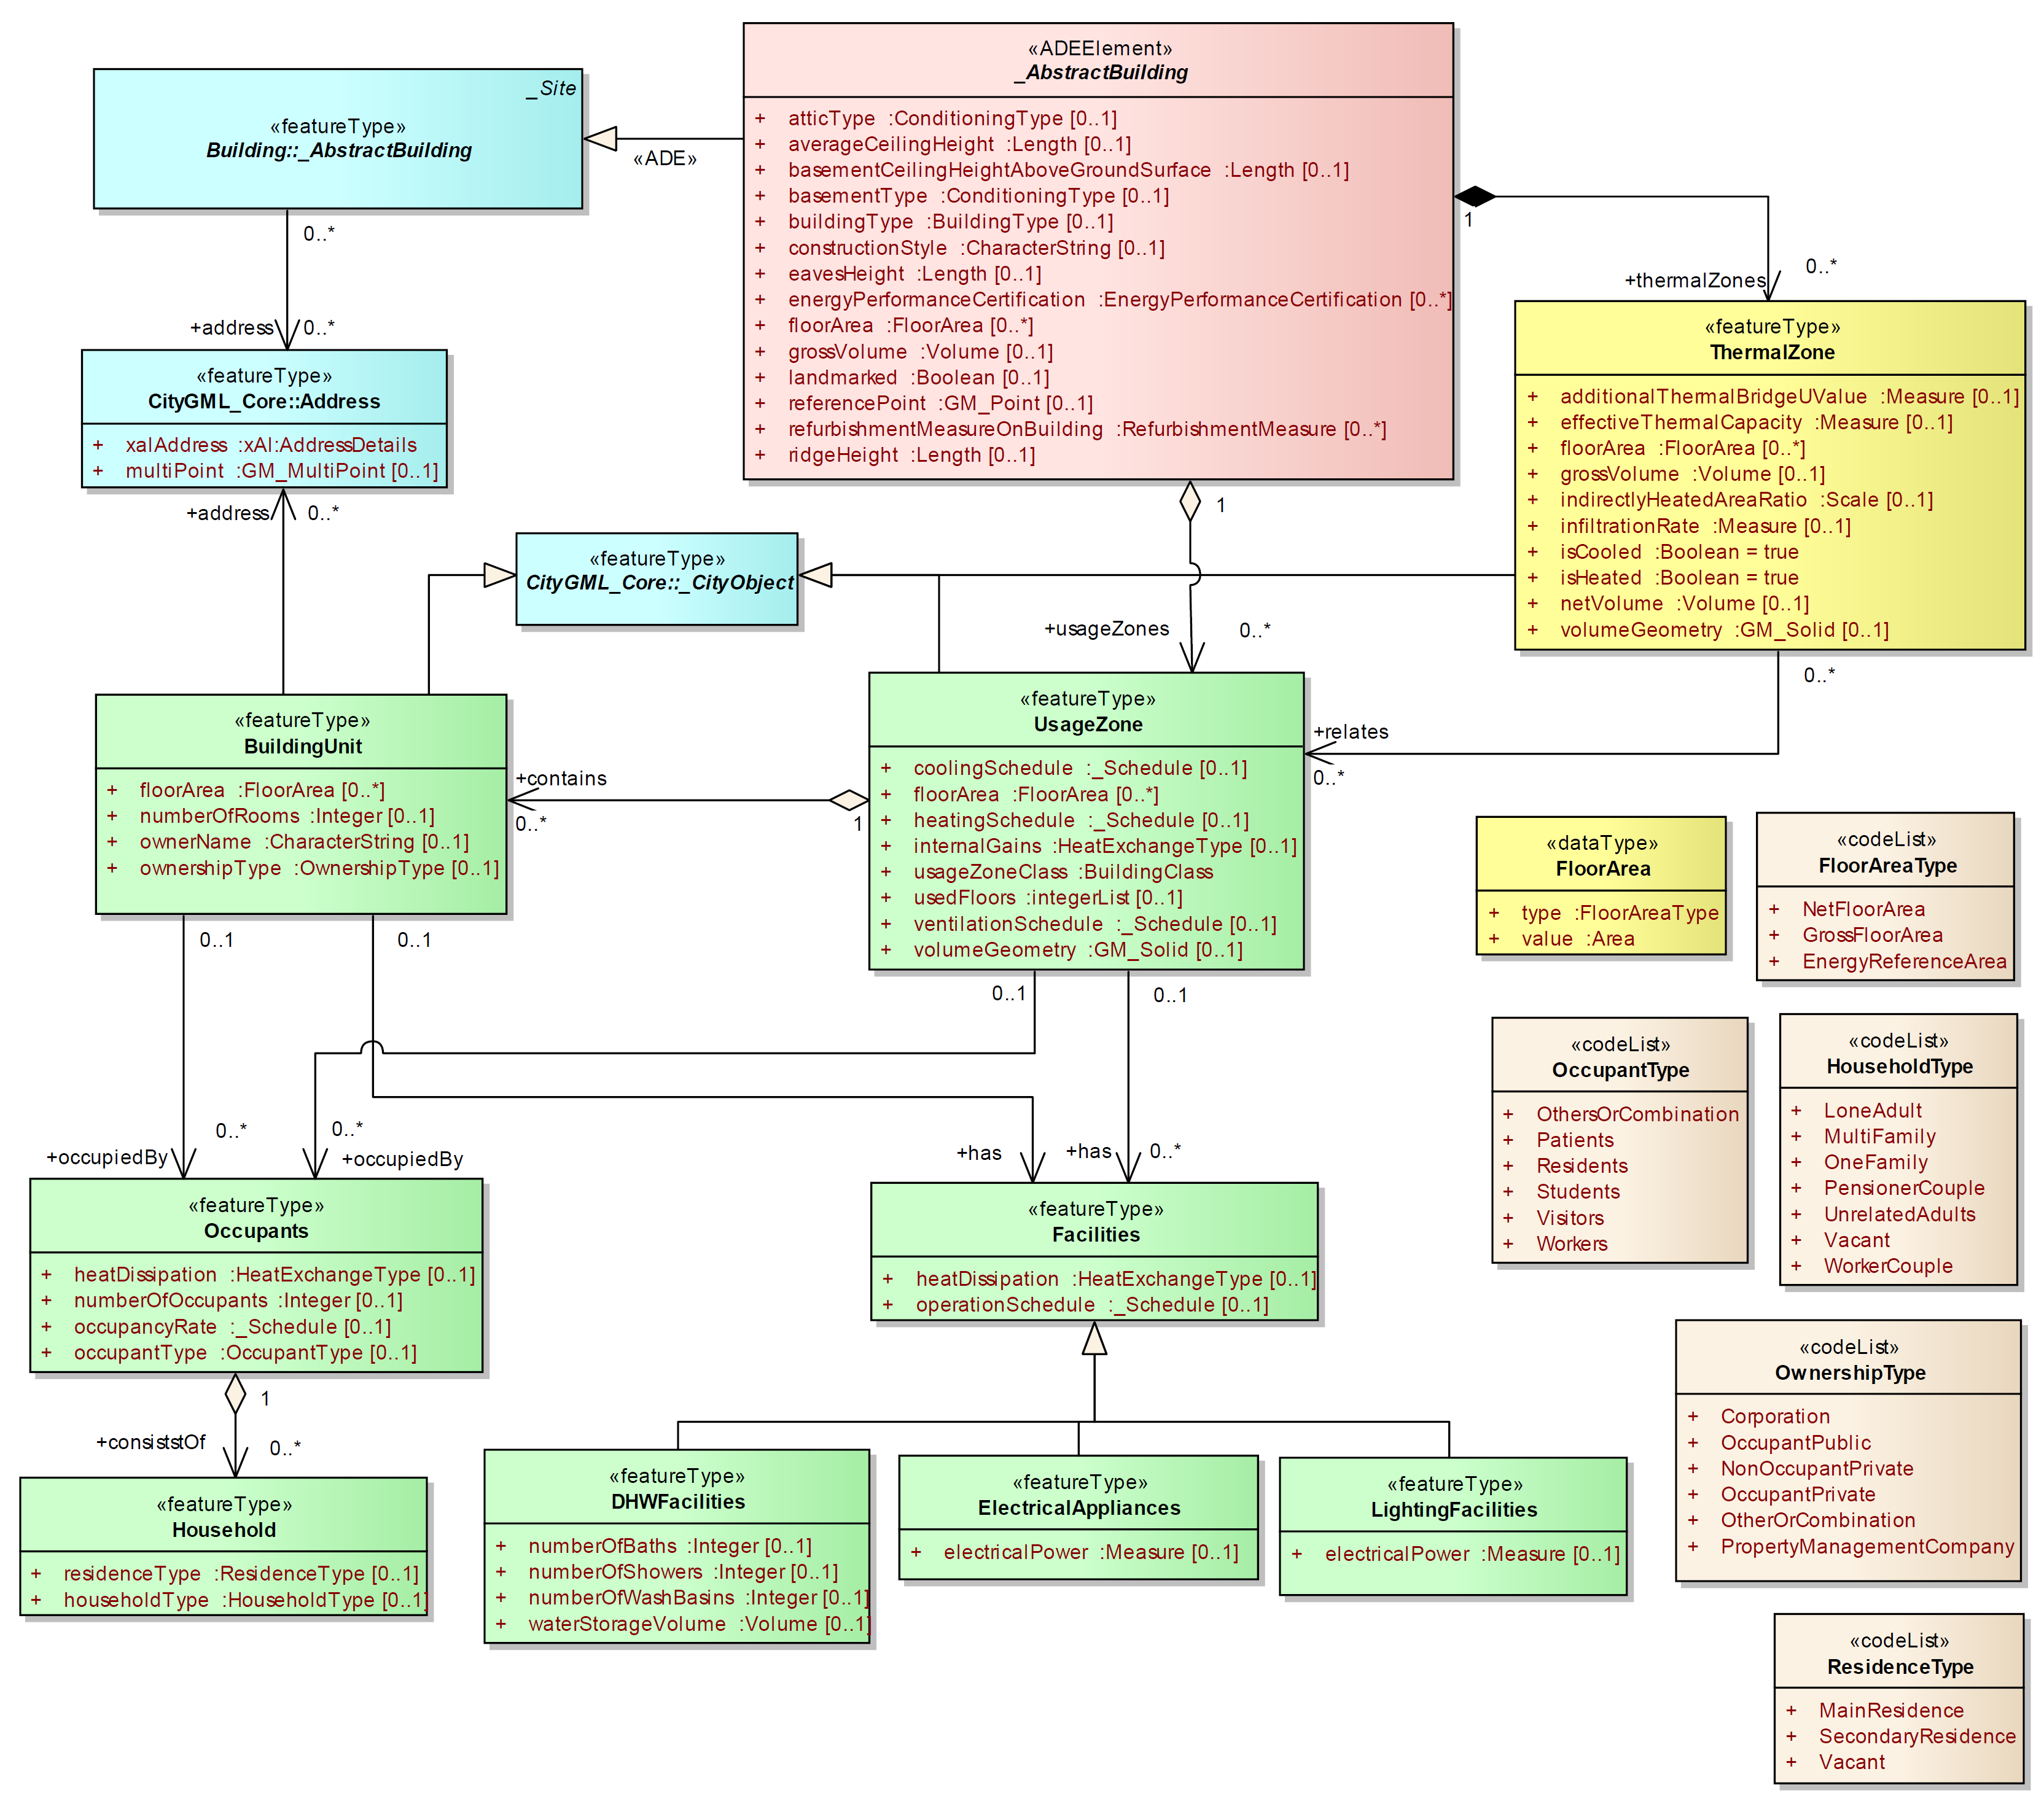
\includegraphics{fig/class_occupancy.png}
\caption{Class diagram of Occupancy Module}
\end{figure}

The Occupancy Module contains the detailed characterization of the
building usage, it is related to the rest of the ADE Energy and CityGML
model through the class \texttt{UsageZone}. Due to the type of
information it allows to store, the Occupancy Module may be used also
for multi-field analysis (socio-economics, demographics etc.).

\subsection{UsageZone}\label{usagezone}

Zone of a building with homogeneous usage type. It is a semantic object,
with an optional geometry (\texttt{volumeGeometry}), which may be or not
related to a geometric entity (Building, BuildingPart, Room etc.).

Its usage type is defined by a \texttt{usageZoneClass} (corresponding to
the CityGML Code list of the \texttt{\_AbstractBuilding} attribute
class). This zone is operated with a single heating and cooling
set-point temperature schedule (\texttt{heatingSchedule} respectively
\texttt{coolingSchedule}) and single air ventilation schedule.

This class inherits from \texttt{\_CityObject} and may therefore be
associated to 1 or more \texttt{EnergyDemand} objects. This class is
defined by at least a usage zone class and a floor area. The building
storeys occupied by this UsageZone may be also indicated by means of the
attribute usedFloorNumbers, e.g.~with 0 corresponding to the ground
floor. Its internalGains attribute corresponds to the sum of the energy
dissipated from the occupants and the facilities inside the zone.

\begin{Shaded}
\begin{Highlighting}[]
\CommentTok{<!--Example of a UsageZone-->}
\KeywordTok{<energy:UsageZone}\OtherTok{ gml:id=}\StringTok{"id_usagezone_1"}\KeywordTok{>}
    \KeywordTok{<gml:description>}\NormalTok{Description of UsageZone 1}\KeywordTok{</gml:description>}
    \KeywordTok{<gml:name>}\NormalTok{Name of UsageZone 1}\KeywordTok{</gml:name>}
    \KeywordTok{<energy:usageZoneClass>}\NormalTok{Commercial}\KeywordTok{</energy:usageZoneClass>}
    \KeywordTok{<energy:usedFloors>}\NormalTok{1}\KeywordTok{</energy:usedFloors>}
    \KeywordTok{<energy:floorArea>}
        \KeywordTok{<energy:FloorArea>}
            \KeywordTok{<energy:type>}\NormalTok{NetFloorArea}\KeywordTok{</energy:type>}
            \KeywordTok{<energy:value>}\NormalTok{40}\KeywordTok{</energy:value>}
        \KeywordTok{</energy:FloorArea>}
    \KeywordTok{</energy:floorArea>}
    \KeywordTok{<energy:internalGains>}
        \KeywordTok{<energy:HeatExchangeType>}
            \KeywordTok{<energy:convectiveFraction}\OtherTok{ uom=}\StringTok{"ratio"}\KeywordTok{>}\NormalTok{0.6}\KeywordTok{</energy:convectiveFraction>}
            \KeywordTok{<energy:latentFraction}\OtherTok{ uom=}\StringTok{"ratio"}\KeywordTok{>}\NormalTok{0.1}\KeywordTok{</energy:latentFraction>}
            \KeywordTok{<energy:radiantFraction}\OtherTok{ uom=}\StringTok{"ratio"}\KeywordTok{>}\NormalTok{0.3}\KeywordTok{</energy:radiantFraction>}
            \KeywordTok{<energy:totalValue}\OtherTok{ uom=}\StringTok{"kW/m^2"}\KeywordTok{>}\NormalTok{80}\KeywordTok{</energy:totalValue>}
        \KeywordTok{</energy:HeatExchangeType>}
    \KeywordTok{</energy:internalGains>}

    \CommentTok{<!--Here follow all BuildingUnit objects, each inside a "contains" tag-->}
    \KeywordTok{<energy:contains>}
        \KeywordTok{<energy:BuildingUnit}\OtherTok{ gml:id=}\StringTok{"id_buildingunit_1"}\KeywordTok{>}
            \CommentTok{<!--Here come all attributes of the first BuildingUnit (if needed) -->}
        \KeywordTok{</energy:BuildingUnit>}
    \KeywordTok{</energy:contains>}
    \CommentTok{<!--Add more BuildingUnit objects here (if needed) -->}

    \CommentTok{<!--Here follow all Occupants objects, each inside a "occupiedBy" tag-->}
    \KeywordTok{<energy:occupiedBy>}
        \KeywordTok{<energy:Occupants}\OtherTok{ gml:id=}\StringTok{"id_occupants_1"}\KeywordTok{>}
            \CommentTok{<!--Here come all attributes of the Occupants object -->}
        \KeywordTok{</energy:Occupants>}
    \KeywordTok{</energy:occupiedBy>}

    \CommentTok{<!--Here follow all Facility objects, each inside a "has" tag-->}
    \KeywordTok{<energy:has>}
        \KeywordTok{<energy:DHWFacilities}\OtherTok{ gml:id=}\StringTok{"id_dhwfacilities_1"}\KeywordTok{>}
            \CommentTok{<!--Here come all attributes of a Facility object -->}
        \KeywordTok{</energy:ElectricalAppliances>}
    \KeywordTok{</energy:has>}
    \KeywordTok{<energy:has>}
        \KeywordTok{<energy:ElectricalAppliances}\OtherTok{ gml:id=}\StringTok{"id_electricalappliance_1"}\KeywordTok{>}
            \CommentTok{<!--Here come all attributes of a Facility object -->}
        \KeywordTok{</energy:ElectricalAppliances>}
    \KeywordTok{</energy:has>}
    \KeywordTok{<energy:has>}
        \KeywordTok{<energy:LightingFacilities}\OtherTok{ gml:id=}\StringTok{"id_lightingfacility_1"}\KeywordTok{>}
            \CommentTok{<!--Here come all attributes of the Facility object -->}
        \KeywordTok{</energy:LightingFacilities>}
    \KeywordTok{</energy:has>}

\KeywordTok{</energy:UsageZone>}
\end{Highlighting}
\end{Shaded}

TODO: Add examples of cooling, heating and ventilation schedules.

\subsection{BuildingUnit}\label{buildingunit}

A \texttt{BuildingUnit} is a part of a \texttt{UsageZone} which is
related to a single occupant entity, such as a dwelling or a workplace.
Owner information attributes (as owner name and ownership type) are
specified in this class. It inherits from class \texttt{\_CityObject}.

\begin{Shaded}
\begin{Highlighting}[]
\CommentTok{<!--Example of a BuildingUnit-->}
\KeywordTok{<energy:BuildingUnit}\OtherTok{ gml:id=}\StringTok{"id_building_unit_1"}\KeywordTok{>}
    \KeywordTok{<gml:description>}\NormalTok{Description of Building Unit 1}\KeywordTok{</gml:description>}
    \KeywordTok{<gml:name>}\NormalTok{Name of Building Unit 1}\KeywordTok{</gml:name>}

    \KeywordTok{<energy:numberOfRooms>}\NormalTok{2}\KeywordTok{</energy:numberOfRooms>}
    \KeywordTok{<energy:ownerName>}\NormalTok{Lilli's Donuts}\KeywordTok{</energy:ownerName>}
    \KeywordTok{<energy:ownershipType>}\NormalTok{OccupantPrivate}\KeywordTok{</energy:ownershipType>}

    \KeywordTok{<energy:floorArea>}
        \KeywordTok{<energy:FloorArea>}
            \KeywordTok{<energy:type>}\NormalTok{NetFloorArea}\KeywordTok{</energy:type>}
            \KeywordTok{<energy:value}\OtherTok{ uom=}\StringTok{"m^2"}\KeywordTok{>}\NormalTok{40}\KeywordTok{</energy:value>}
        \KeywordTok{</energy:FloorArea>}
    \KeywordTok{</energy:floorArea>}

    \CommentTok{<!--Here follow all Occupants objects, each inside a "occupiedBy" tag-->}
    \KeywordTok{<energy:occupiedBy>}
        \KeywordTok{<energy:Occupants}\OtherTok{ gml:id=}\StringTok{"id_occupants_1"}\KeywordTok{>}
            \CommentTok{<!--Here come all attributes of the Occupants object -->}
        \KeywordTok{</energy:Occupants>}
    \KeywordTok{</energy:occupiedBy>}

    \CommentTok{<!--Here follow all Facility objects, each inside a "has" tag-->}
    \KeywordTok{<energy:has>}
        \KeywordTok{<energy:DHWFacilities}\OtherTok{ gml:id=}\StringTok{"id_dhwfacilities_1"}\KeywordTok{>}
            \CommentTok{<!--Here come all attributes of a Facility object -->}
        \KeywordTok{</energy:DHWFacilities>}
    \KeywordTok{</energy:has>}

\KeywordTok{</energy:BuildingUnit>}
\end{Highlighting}
\end{Shaded}

\subsection{Occupants}\label{occupants}

An \texttt{Occupants} class identifies a homogeneous group of occupants
of a usage zone or building unit, defined with an occupant type
(e.g.~residents, workers, visitors etc.). It can optionally contain one
or more Household objects.

\begin{Shaded}
\begin{Highlighting}[]
\CommentTok{<!--Example of a Occupants object-->}
\KeywordTok{<energy:Occupants}\OtherTok{ gml:id=}\StringTok{"id_occupants_1"}\KeywordTok{>}
    \KeywordTok{<gml:description>}\NormalTok{Description of Occupants 1}\KeywordTok{</gml:description>}
    \KeywordTok{<gml:name>}\NormalTok{Name of Occupants 1}\KeywordTok{</gml:name>}

    \KeywordTok{<energy:heatDissipation>}
        \KeywordTok{<energy:HeatExchangeType>}
            \KeywordTok{<energy:convectiveFraction}\OtherTok{ uom=}\StringTok{"ratio"}\KeywordTok{>}\NormalTok{0.1}\KeywordTok{</energy:convectiveFraction>}
            \KeywordTok{<energy:latentFraction}\OtherTok{ uom=}\StringTok{"ratio"}\KeywordTok{>}\NormalTok{0.1}\KeywordTok{</energy:latentFraction>}
            \KeywordTok{<energy:radiantFraction}\OtherTok{ uom=}\StringTok{"ratio"}\KeywordTok{>}\NormalTok{0.8}\KeywordTok{</energy:radiantFraction>}
            \KeywordTok{<energy:totalValue}\OtherTok{ uom=}\StringTok{"W/person"}\KeywordTok{>}\NormalTok{80}\KeywordTok{</energy:totalValue>}
        \KeywordTok{</energy:HeatExchangeType>}
    \KeywordTok{</energy:heatDissipation>}

    \KeywordTok{<energy:numberOfOccupants>}\NormalTok{3}\KeywordTok{</energy:numberOfOccupants>}

    \KeywordTok{<energy:occupancyRate>}
        \CommentTok{<!--Add here the Schedule data -->}
    \KeywordTok{</energy:occupancyRate>}

    \KeywordTok{<energy:occupantType>}\NormalTok{Residents}\KeywordTok{</energy:occupantType>}

    \CommentTok{<!--Here follow all Household objects, each inside a "consistsOf" tag-->}
    \KeywordTok{<energy:consiststOf>}
        \KeywordTok{<energy:Household}\OtherTok{ gml:id=}\StringTok{"id_household_1"}\KeywordTok{>}
            \CommentTok{<!--Here come all attributes of the first Household (omitted here)-->}
        \KeywordTok{</energy:Household>}
    \KeywordTok{</energy:consiststOf>}
    \KeywordTok{<energy:consiststOf>}
        \KeywordTok{<energy:Household}\OtherTok{ gml:id=}\StringTok{"id_household_2"}\KeywordTok{>}
            \CommentTok{<!--Here come all attributes of the second Household (omitted here)-->}
        \KeywordTok{</energy:Household>}
    \KeywordTok{</energy:consiststOf>}

\KeywordTok{</energy:Occupants>}
\end{Highlighting}
\end{Shaded}

\subsection{Household}\label{household}

A \texttt{Household} class identifies a group of persons living in the
same dwelling, in the case where occupants are residents. They are
defined by a type (e.g.~one family, worker couple, etc.) and a residence
type (main/secondary residence or vacant).

\begin{Shaded}
\begin{Highlighting}[]
\CommentTok{<!--Example of a Household object-->}
\KeywordTok{<energy:Household}\OtherTok{ gml:id=}\StringTok{"id_household_1"}\KeywordTok{>}
    \KeywordTok{<gml:description>}\NormalTok{Description of Household 1}\KeywordTok{</gml:description>}
    \KeywordTok{<gml:name>}\NormalTok{Name of Household 1}\KeywordTok{</gml:name>}
    \KeywordTok{<energy:residenceType>}\NormalTok{SecondaryResidence}\KeywordTok{</energy:residenceType>}
    \KeywordTok{<energy:householdType>}\NormalTok{UnrelatedAdults}\KeywordTok{</energy:householdType>}
\KeywordTok{</energy:Household>}
\end{Highlighting}
\end{Shaded}

\subsection{Facilities}\label{facilities}

Each \texttt{UsageZone} or \texttt{BuildingUnit} object can have one or
multiple \texttt{Facilities} objects. Currently there are three types of
facilities (DHWFacilities, ElectricalAppliances and LightingFacilities).
Each of them is characterised by the heatDissipation and the
operationSchedule attributes, plus some specific ones depending on the
facility type. In the following, two XML examples are presented, one for
domestic how water facilities and one for electrical applicances. Please
note that the lighting facilities object shares the same structure and
attributes of the ElectricalAppliances.

\begin{Shaded}
\begin{Highlighting}[]
\CommentTok{<!--Example of a DHWFacilities object-->}
\KeywordTok{<energy:DHWFacilities}\OtherTok{ gml:id=}\StringTok{"id_dhwfacilities_1"}\KeywordTok{>}
    \KeywordTok{<gml:description>}\NormalTok{Description of Domestic Hot Water Facilities 1}\KeywordTok{</gml:description>}
    \KeywordTok{<gml:name>}\NormalTok{Name of Domestic Hot Water Facilities 1}\KeywordTok{</gml:name>}

    \KeywordTok{<energy:heatDissipation>}
        \KeywordTok{<energy:HeatExchangeType>}
            \KeywordTok{<energy:convectiveFraction}\OtherTok{ uom=}\StringTok{"ratio"}\KeywordTok{>}\NormalTok{0.5}\KeywordTok{</energy:convectiveFraction>}
            \KeywordTok{<energy:latentFraction}\OtherTok{ uom=}\StringTok{"ratio"}\KeywordTok{>}\NormalTok{0.3}\KeywordTok{</energy:latentFraction>}
            \KeywordTok{<energy:radiantFraction}\OtherTok{ uom=}\StringTok{"ratio"}\KeywordTok{>}\NormalTok{0.2}\KeywordTok{</energy:radiantFraction>}
            \KeywordTok{<energy:totalValue}\OtherTok{ uom=}\StringTok{"W/m^2"}\KeywordTok{>}\NormalTok{10}\KeywordTok{</energy:totalValue>}
        \KeywordTok{</energy:HeatExchangeType>}
    \KeywordTok{</energy:heatDissipation>}

    \KeywordTok{<energy:operationSchedule>}
        \CommentTok{<!--Add here the Schedule data -->}
    \KeywordTok{</energy:operationSchedule>}

    \KeywordTok{<energy:numberOfBaths>}\NormalTok{1}\KeywordTok{</energy:numberOfBaths>}
    \KeywordTok{<energy:numberOfShowers>}\NormalTok{0}\KeywordTok{</energy:numberOfShowers>}
    \KeywordTok{<energy:numberOfWashBasins>}\NormalTok{1}\KeywordTok{</energy:numberOfWashBasins>}
    \KeywordTok{<energy:waterStorageVolume}\OtherTok{ uom=}\StringTok{"m^3"}\KeywordTok{>}\NormalTok{0.8}\KeywordTok{</energy:waterStorageVolume>}
\KeywordTok{</energy:DHWFacilities>}
\end{Highlighting}
\end{Shaded}

\begin{Shaded}
\begin{Highlighting}[]
\CommentTok{<!--Example of an ElectricalApplicances object-->}
\KeywordTok{<energy:ElectricalAppliances}\OtherTok{ gml:id=}\StringTok{"id_electricalappliance_1"}\KeywordTok{>}
    \KeywordTok{<gml:description>}\NormalTok{Description of Electrical Applicance 1}\KeywordTok{</gml:description>}
    \KeywordTok{<gml:name>}\NormalTok{Name of Electrical Applicance 1}\KeywordTok{</gml:name>}

    \KeywordTok{<energy:heatDissipation>}
        \KeywordTok{<energy:HeatExchangeType>}
            \KeywordTok{<energy:totalValue}\OtherTok{ uom=}\StringTok{"W/m^2"}\KeywordTok{>}\NormalTok{10}\KeywordTok{</energy:totalValue>}
        \KeywordTok{</energy:HeatExchangeType>}
    \KeywordTok{</energy:heatDissipation>}

    \KeywordTok{<energy:electricalPower}\OtherTok{ uom=}\StringTok{"kW"}\KeywordTok{>}\NormalTok{1}\KeywordTok{</energy:electricalPower>}

    \KeywordTok{<energy:operationSchedule>}
        \CommentTok{<!--Add here the Schedule data -->}
    \KeywordTok{</energy:operationSchedule>}

\KeywordTok{</energy:ElectricalAppliances>}
\end{Highlighting}
\end{Shaded}

\section{Energy System Module}\label{energy-system-module}

\begin{figure}[htbp]
\centering
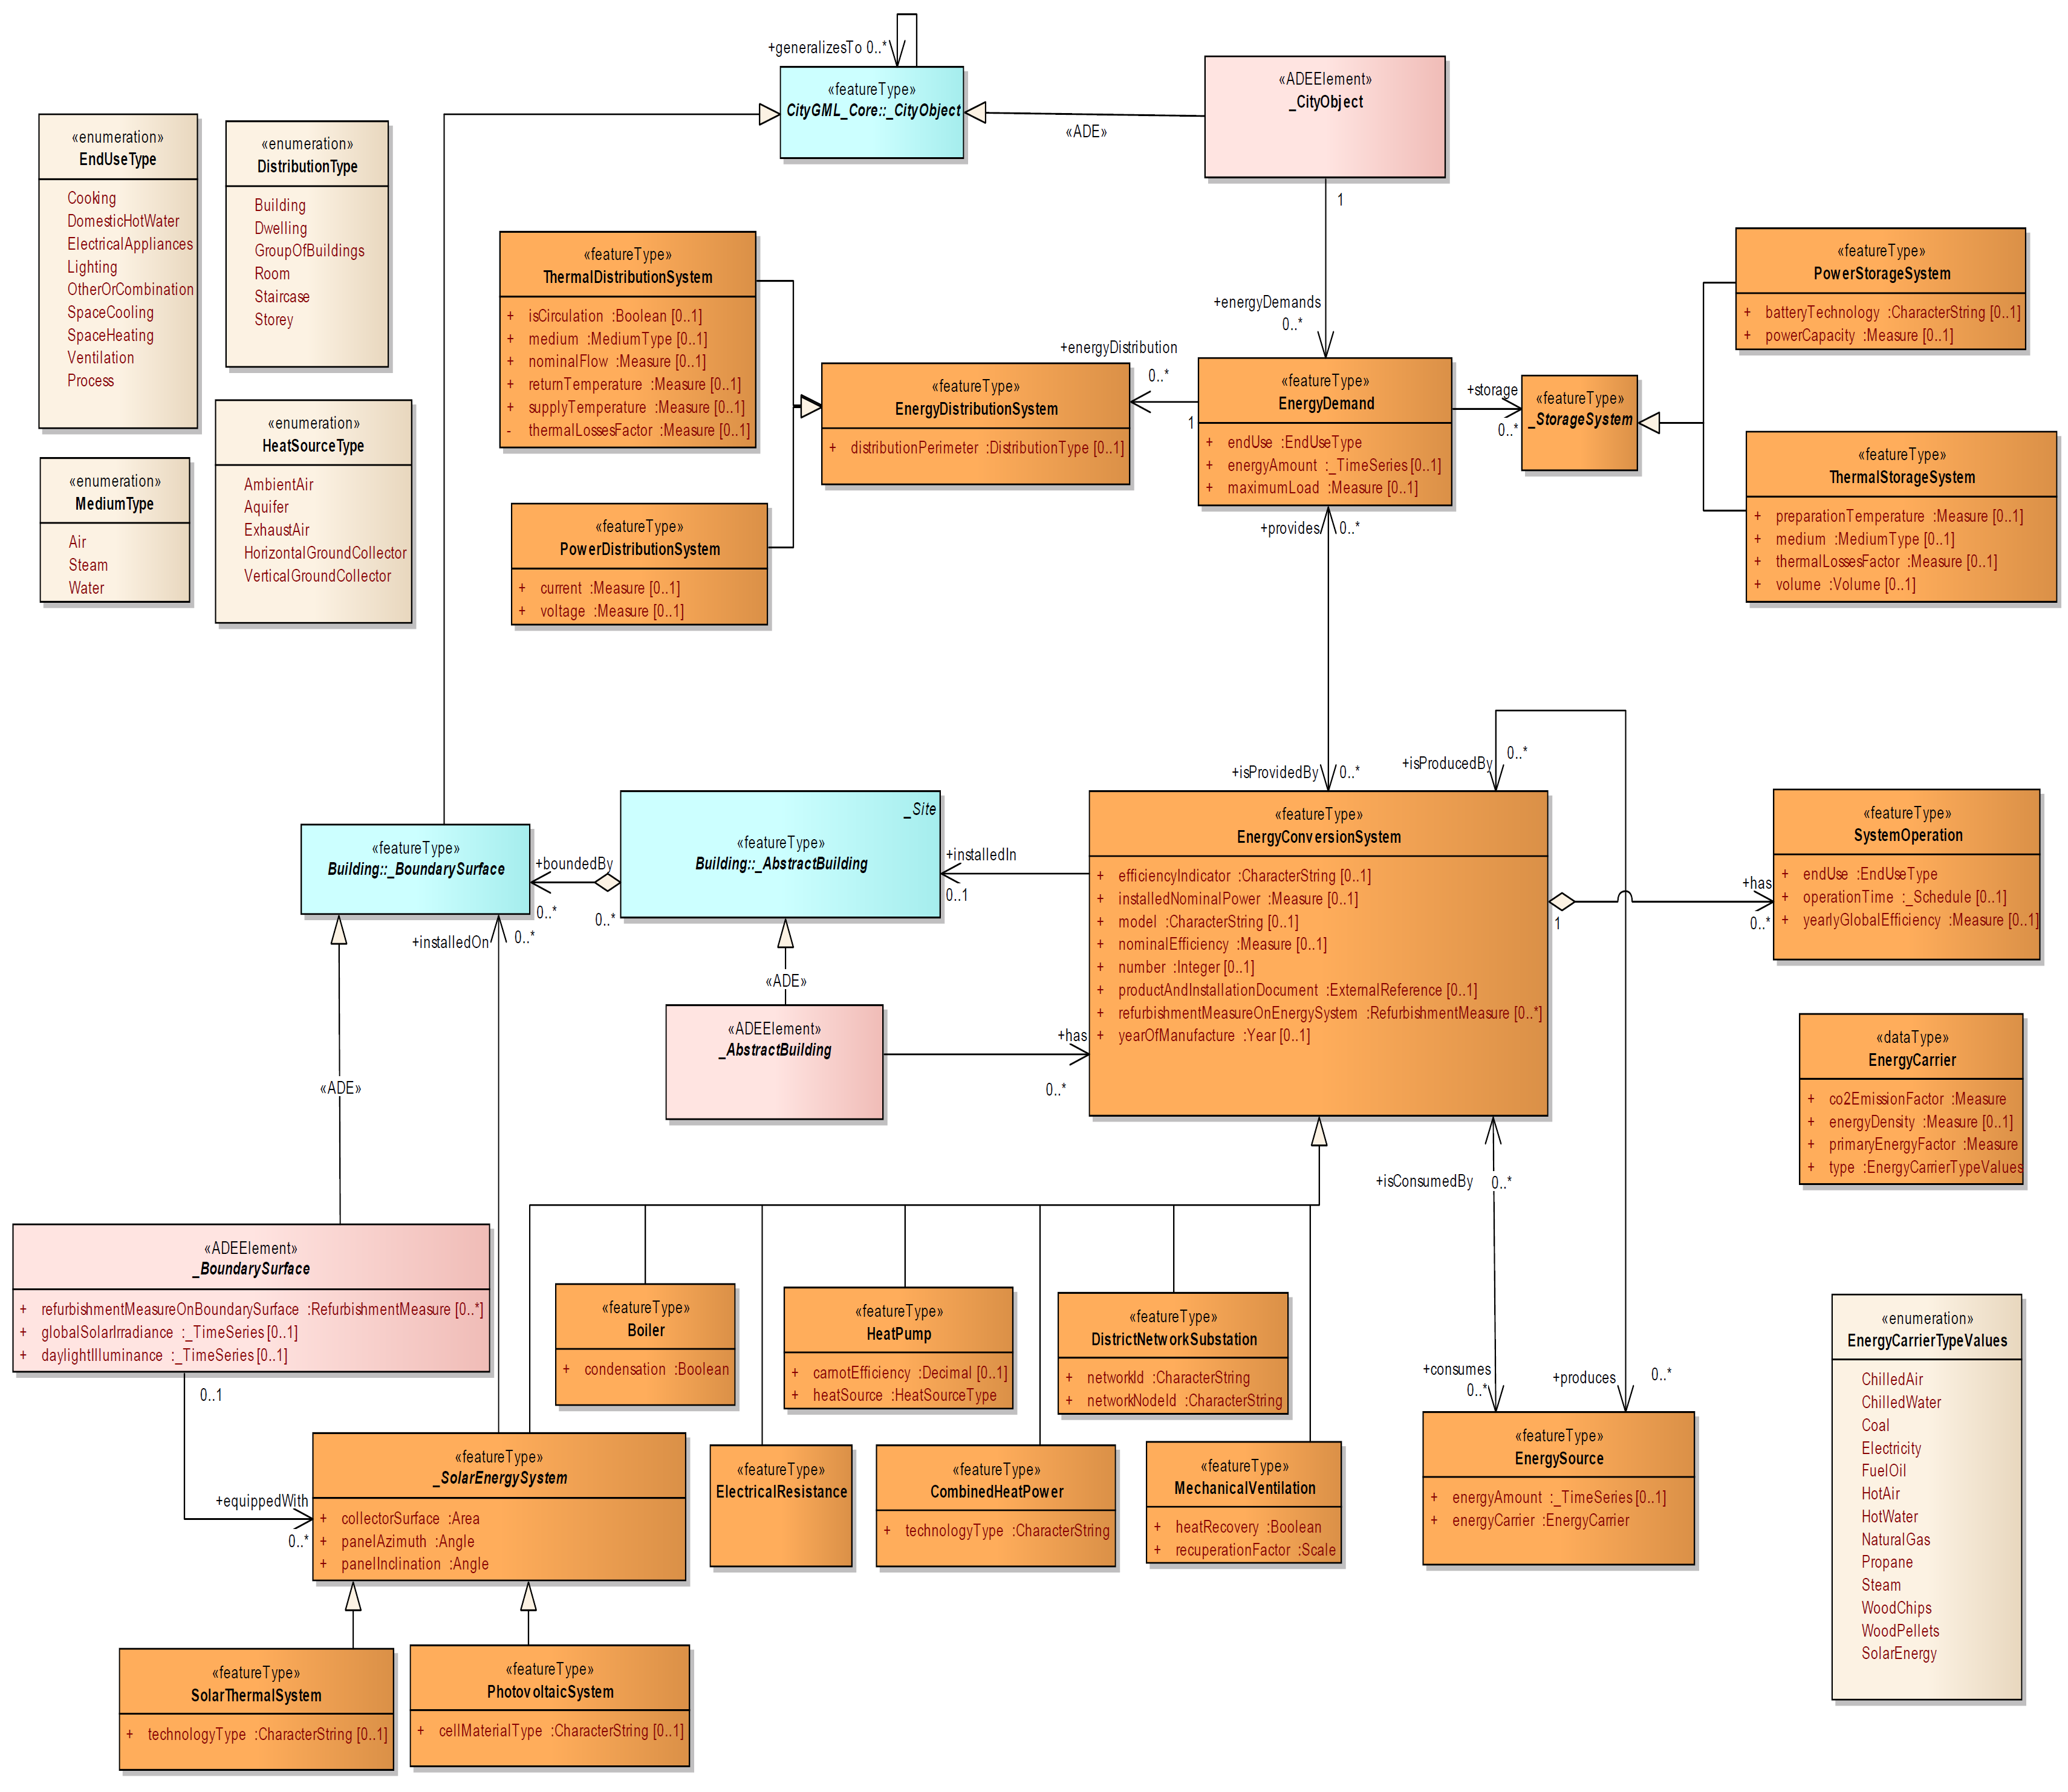
\includegraphics{fig/class_EnergySystem.png}
\caption{Class diagram of Energy System Module}
\end{figure}

The Energy System Module is a module of the ADE Energy which contains
information concerning the energy forms (energy demand, supply, sources)
and the energy systems (conversion, distribution and storage systems).
It is arranged around one central \texttt{EnergyDemand} object.

\subsection{EnergyDemand}\label{energydemand}

Useful energy required to satisfy a specific end use, such as heating,
cooling, domestic hot water etc. Beside its \texttt{EndUseType}, this
object is characterized its \texttt{energyAmount} (time-depending energy
demand value) and its maximum yearly load (\texttt{maximumLoad}) used
for the sizing of the energy systems.

Every \texttt{\_CityObject} (typically \texttt{ADE:\_AbstractBuilding},
\texttt{ThermalZone}, \texttt{UsageZone} and \texttt{BuildingUnit}) may
have one or more \texttt{EnergyDemand}.

\subsubsection{EndUseType}\label{endusetype}

List of possible end uses as cooking, space heating and ventilation.

\subsubsection{EnergySource}\label{energysource}

Final energy consumed (and sometimes produced) by the energy conversion
system. Its energy characteristics are specified in the Energy Carrier
object.

\subsubsection{EnergyCarrier}\label{energycarrier}

Primary energy and \(CO_2\) emission factors, energy density and energy
carrier type characterize this data type for energy carriers.

\subsubsection{EnergyCarrierType}\label{energycarriertype}

List of energy carriers as coal, chilled water or electricity.

\subsection{Energy Distribution}\label{energy-distribution}

\subsubsection{EnergyDistributionSystem}\label{energydistributionsystem}

System in charge of delivering the energy inside the building, from the
place of energy production to the place of end-use. Power and Thermal
distribution systems are differentiated. They all share a distribution
perimeter that is described by the distribution type.

\subsubsection{Distribution Type}\label{distribution-type}

A list of possible distribution perimeters, e.g.~Building, Dwelling,
Room.

\subsubsection{ThermalDistributionSystem}\label{thermaldistributionsystem}

Type for thermal distribution systems with attributes for circulation
(circulating system or not), the used medium, nominal flow, return and
supply temperatures and thermal losses factor.

\subsubsection{PowerDistributionSystem}\label{powerdistributionsystem}

Type for electrical distribution systems, described by current and
voltage.

\subsubsection{MediumType}\label{mediumtype}

This list is a collection of medium types as air and water.

\subsection{Energy Storage}\label{energy-storage}

\subsubsection{StorageSystem}\label{storagesystem}

System storing energy. A same storage may store the energy of different
end-users and different end uses. Power and Thermal storage systems are
differentiated.

\subsubsection{ThermalStorageSystem}\label{thermalstoragesystem}

Thermal storages with a medium, preparation temperature, thermal losses
factor and a volume.

\subsubsection{PowerStorageSystem}\label{powerstoragesystem}

Electrical storages with an electrical capacity and a string to describe
the battery technology.

\subsection{Energy Conversion}\label{energy-conversion}

\subsubsection{EnergyConversionSystem}\label{energyconversionsystem}

System converting an energy source into the energy necessary to satisfy
the \texttt{EnergyDemand} (or to feed the networks).

Energy conversion systems have common parameters: efficiency indicator,
nominal installed power, nominal efficiency (in reference to an
efficiency indicator), year of manufacture, name of the model, a serial
number, a reference to product or installation documents and optionally
refurbishment measures. They may be one or more (in this case, the
nominal installed power corresponds to the totality).

Specific energy conversion systems may have in addition specific
parameters:

A same system may have several operation modes (e.g.~heat pump covering
heating and domestic hot water demands).

\subsubsection{SystemOperation}\label{systemoperation}

It details the operation of the energy conversion system for a specific
end-use and operation time. For instance, a reversible heat pump may
have 3 operation modes: heating production in winter, cooling production
in summer, and hot water production during the whole year. Attributes
are end use type, a schedule for operation time and yearly global
efficiency.

\subsubsection{DistrictNetworkSubstation}\label{districtnetworksubstation}

Subtype of \texttt{EnergyConversionSystem} for heating or cooling
networks substations. Adds attributes for network ID and network node
ID.

\subsubsection{HeatPump}\label{heatpump}

Subtype of \texttt{EnergyConversionSystem} for heat pumps to add carnot
efficiency and heat source. Heat source is described using a
\texttt{HeatSourceType}.

\subsubsection{HeatSourceType}\label{heatsourcetype}

List of heat source types for heat pumps, e.g.~ambient air, aquifer and
exhaust air.

\subsubsection{ElectricalResistance}\label{electricalresistance}

Subtype of \texttt{EnergyConversionSystem} for electrical resistances.
Comes without additional attributes.

\subsubsection{MechanicalVentilation}\label{mechanicalventilation}

Subtype of \texttt{EnergyConversionSystem} for ventilation systems with
attributes heat recovery (with or without) and recuperation factor.

\subsubsection{CombinedHeatPower}\label{combinedheatpower}

Subtype of \texttt{EnergyConversionSystem} for CHP systems. Utilizes a
string describing the technology type.

\subsubsection{Boiler}\label{boiler}

Subtype of \texttt{EnergyConversionSystem} for boiler. Defines if it is
a condensation boiler or not.

\subsubsection{SolarEnergySystem}\label{solarenergysystem}

Subclass of \texttt{EnergyConversionSystem} for solar energy systems.
Has attributes for collector surface, azimuth and inclination.
Differentiates into solar thermal and photovoltaic systems.

\subsubsection{SolarThermalSystem}\label{solarthermalsystem}

Subtype of \texttt{SolarEnergySystem} for thermal systems. Uses a string
to describe the technology type.

\subsubsection{PhotovoltaicSystem}\label{photovoltaicsystem}

Subtype of \texttt{SolarEnergySystem} for photovoltaic systems. Defines
the material type of photovoltaic cells with a string.

\section*{References}\label{references}
\addcontentsline{toc}{section}{References}

\hypertarget{refs}{}

\end{document}
